\documentclass[12pt,a4paper,]{article}
\usepackage[]{mathpazo}
\usepackage{setspace}
\setstretch{2}
\usepackage{amssymb,amsmath}
\usepackage{ifxetex,ifluatex}
\usepackage{fixltx2e} % provides \textsubscript
\ifnum 0\ifxetex 1\fi\ifluatex 1\fi=0 % if pdftex
  \usepackage[T1]{fontenc}
  \usepackage[utf8]{inputenc}
\else % if luatex or xelatex
  \ifxetex
    \usepackage{mathspec}
  \else
    \usepackage{fontspec}
  \fi
  \defaultfontfeatures{Ligatures=TeX,Scale=MatchLowercase}
\fi
% use upquote if available, for straight quotes in verbatim environments
\IfFileExists{upquote.sty}{\usepackage{upquote}}{}
% use microtype if available
\IfFileExists{microtype.sty}{%
\usepackage[]{microtype}
\UseMicrotypeSet[protrusion]{basicmath} % disable protrusion for tt fonts
}{}
\PassOptionsToPackage{hyphens}{url} % url is loaded by hyperref
\usepackage[unicode=true]{hyperref}
\PassOptionsToPackage{usenames,dvipsnames}{color} % color is loaded by hyperref
\hypersetup{
            pdftitle={Trade-offs among plant floral and reproductive traits determine interactions with floral visitors},
            pdfauthor={Jose B. Lanuza1,2*; Romina Rader1; Jamie Stavert3; Liam K. Kendall4; Manu E. Saunders1; Ignasi Bartomeus2},
            colorlinks=true,
            linkcolor=RoyalBlue,
            citecolor=Blue,
            urlcolor=RoyalBlue,
            breaklinks=true}
\urlstyle{same}  % don't use monospace font for urls
\usepackage[margin=1in]{geometry}
\usepackage{longtable,booktabs}
% Fix footnotes in tables (requires footnote package)
\IfFileExists{footnote.sty}{\usepackage{footnote}\makesavenoteenv{long table}}{}
\usepackage{graphicx,grffile}
\makeatletter
\def\maxwidth{\ifdim\Gin@nat@width>\linewidth\linewidth\else\Gin@nat@width\fi}
\def\maxheight{\ifdim\Gin@nat@height>\textheight\textheight\else\Gin@nat@height\fi}
\makeatother
% Scale images if necessary, so that they will not overflow the page
% margins by default, and it is still possible to overwrite the defaults
% using explicit options in \includegraphics[width, height, ...]{}
\setkeys{Gin}{width=\maxwidth,height=\maxheight,keepaspectratio}
\IfFileExists{parskip.sty}{%
\usepackage{parskip}
}{% else
\setlength{\parindent}{0pt}
\setlength{\parskip}{6pt plus 2pt minus 1pt}
}
\setlength{\emergencystretch}{3em}  % prevent overfull lines
\providecommand{\tightlist}{%
  \setlength{\itemsep}{0pt}\setlength{\parskip}{0pt}}
\setcounter{secnumdepth}{0}
% Redefines (sub)paragraphs to behave more like sections
\ifx\paragraph\undefined\else
\let\oldparagraph\paragraph
\renewcommand{\paragraph}[1]{\oldparagraph{#1}\mbox{}}
\fi
\ifx\subparagraph\undefined\else
\let\oldsubparagraph\subparagraph
\renewcommand{\subparagraph}[1]{\oldsubparagraph{#1}\mbox{}}
\fi

% set default figure placement to htbp
\makeatletter
\def\fps@figure{htbp}
\makeatother

\usepackage{lineno} % add 
\linenumbers % turns line numbering on 

% Allowing for landscape pages
\usepackage{lscape}
\newcommand{\blandscape}{\begin{landscape}}
\newcommand{\elandscape}{\end{landscape}}

% Left justification of the text: see https://www.sharelatex.com/learn/Text_alignment
% \usepackage[document]{ragged2e} % already in the latex template
\newcommand{\bleft}{\begin{flushleft}}
\newcommand{\eleft}{\end{flushleft}}


% Add Supplementary Tables and Figures
% Code from https://stackoverflow.com/a/51337664
\newcommand{\beginsupplement}{
  \setcounter{table}{0}  
  \renewcommand{\thetable}{S\arabic{table}}
  \setcounter{figure}{0} 
  \renewcommand{\thefigure}{S\arabic{figure}}
}
\usepackage{booktabs}
\usepackage{longtable}
\usepackage{array}
\usepackage{multirow}
\usepackage{wrapfig}
\usepackage{float}
\usepackage{colortbl}
\usepackage{pdflscape}
\usepackage{tabu}
\usepackage{threeparttable}
\usepackage{threeparttablex}
\usepackage[normalem]{ulem}
\usepackage{makecell}
\usepackage{xcolor}
\usepackage{float}
\floatplacement{figure}{H}
\usepackage[skip=5pt]{caption}
\usepackage{float}
\usepackage{booktabs}
\usepackage{longtable}
\usepackage{array}
\usepackage{multirow}
\usepackage{wrapfig}
\usepackage{colortbl}
\usepackage{pdflscape}
\usepackage{tabu}
\usepackage{threeparttable}
\usepackage{threeparttablex}
\usepackage[normalem]{ulem}
\usepackage{makecell}
\usepackage{xcolor}

\title{Trade-offs among plant floral and reproductive traits determine
interactions with floral visitors}
\author{Jose B. Lanuza\textsuperscript{1,2}* \and Romina Rader\textsuperscript{1} \and Jamie Stavert\textsuperscript{3} \and Liam K. Kendall\textsuperscript{4} \and Manu E. Saunders\textsuperscript{1} \and Ignasi Bartomeus\textsuperscript{2}}
\date{}

\begin{document}
\maketitle

\small

\textsuperscript{1} School of Environmental and Rural Science,
University of New England, Armidale, New South Wales 2350, Australia

\textsuperscript{2} Estación Biológica de Doñana (EBD-CSIC), E-41092
Seville, Spain

\textsuperscript{3} Department of Conservation \textbar{} Te Papa
Atawhai, Auckland, New Zealand

\textsuperscript{4} Centre for Environmental and Climate Science, Lund
University, Sölvegatan 37, S-223 62 Lund, Sweden

\texttt{*} Corresponding author:
\href{mailto:barragansljose@gmail.com}{\nolinkurl{barragansljose@gmail.com}}

\normalsize

Plant life strategies are often delimited by vegetative and
physiological traits but little is known about how floral and
reproductive traits drive these strategies, and in turn shape plant
interactions with floral visitors. Here, we compiled 13 floral, 4
reproductive and 3 vegetative traits for 1,506 plant species from 28
plant-pollinator network studies across 18 different countries. We
investigated the associations among these traits, pollinator visitation
and the functional role of plant species within the networks
(interaction frequency, normalized degree and specialization). We found
that 51.8\% of trait variation was explained by two independent axes
that encompassed plant form and function. Specifically, the first axis
indicated the presence of a trade-off between flower number and flower
size (PC1, 26.72\%). The second axis indicated a trade-off for the level
of pollinator dependency (PC2, 25.08\%). Although the main axes of trait
variation did not fully explain pollinator visitation rates, different
plant life strategies were associated with visitation rates and
pollinator functional groups. Overall, the main traits that determined
plant species' functional roles were height, nectar concentration,
pollen grains per flower, number of ovules, style length, selfing level
and flower width. Our results highlight the need to consider plant
reproductive and floral traits to improve understanding of plant life
strategies and plant-pollinator interactions at broader spatial scales.

\vspace{5mm} \bleft

There is an astonishing diversity of floral structures and plant
reproductive strategies among flowering plants (Barrett, 2002; Schiestl
\& Johnson, 2013), which have long been of interest to pollination
biologists in terms of their relevance to plant-pollinator interactions.
However, most studies that have explored reproductive (e.g., mating and
compatibility systems) and floral trait (e.g., flower size or nectar
provision) variation have concentrated on the individual or community
level and thus, broader macroecological patterns remain poorly
investigated (Carvalheiro et al., 2014; Baude et al., 2016; Munoz et
al., 2016; Moeller et al., 2017; Grossenbacher et al., 2017). Indeed,
studies depicting species' life history strategies generally focus on
vegetative traits and rarely consider reproductive traits
(Salguero-Gómez et al., 2016; Rüger et al., 2018). As a consequence, a
unified framework that explores the compromises among floral traits and
their relevance to plant life strategies is currently lacking (Roddy et
al., 2021). At the same time, there is growing interest in the
determinants of plant-pollinator interactions via trait-based approaches
(Fenster et al., 2004) and trait-matching analyses (Bartomeus et al.,
2016). However, floral traits have been overlooked beyond highly
specialised plant-pollinator systems (Dellinger, 2020; Roddy et al.,
2021) and the role of plant reproductive biology remains little explored
in plant-pollinator interactions (but see Tur et al., 2013 and Devaux et
al., 2014).

With the recent availability of large trait databases, plant ecological
strategies are increasingly being examined (e.g., TRY, Kattge et al.,
2011 and COMPADRE, Salguero‐Gómez et al., 2015), and are facilitating
the identification of global patterns and constraints of plant form and
function (Salguero‐Gómez et al., 2015; Díaz et al., 2016; Carmona et
al., 2021). However, the main focus has been on vegetative traits such
as leaf (Wright et al., 2004) or wood (Chave et al., 2009) trade-offs
with little or no attention given to reproductive and floral traits
(E‐Vojtkó et al., 2020), also critical to plant form and function. For
instance, short lived versus perennial species tend to have low versus
high levels of outcrossing, respectively (Barrett, 2003; Moeller et al.,
2017). Further, outcrossing levels are positively correlated with flower
size (Goodwillie et al., 2010). In addition, the presence of costly
rewards (e.g., pollen or nectar) and showy flowers or floral displays
can only be understood through consideration of plant species' reliance
upon animal pollination (pollinator dependence) and their role in
attracting pollinators (Ollerton et al., 2011). Hence, exploring plant
life strategies with reproductive and floral trade-offs, in conjunction
with their pollinator dependence, is necessary for a balanced
understanding of plant economics.

Several studies have identified links between plant traits and
plant-pollinator network properties (Lázaro et al., 2008; Bartomeus,
2013; Carvalheiro et al., 2014). Moreover, plant traits can also define
species' network roles (e.g., specialists vs generalists). For example,
species that occupy trait space extremes are more likely to exhibit
higher specialization and be more reliant on trait-matching (Junker et
al., 2013; Coux et al., 2016). This morphological matching between plant
and floral visitors can determine plant-pollinator interactions, and
thus shape their interaction network structure (Stang et al., 2009;
Ibanez, 2012). Despite the increasing knowledge of the relevance of
traits on the species network roles, little is known about how plant
reproductive and floral traits determine plant species' network roles at
a macroecological scale.

Here, we explore the potential trade-offs among plant floral and
reproductive traits and how these influence the structure of
plant-pollinator networks. First, we identify the major axes of floral
and reproductive trait variation and trade-offs that determine plant
form and function. Second, we investigate how plant species' position in
trait-space influences interaction strength with different guilds of
floral visitors. Finally, we investigate how the main axes of trait
variation and individual traits influence plant species roles within
networks using complementary interaction network metrics (i.e.,
interaction strength, normalized degree and specialization).

\section{RESULTS}\label{results}

\textbf{Plant strategies}

The phylogenetically informed principal component analysis (pPCA)
captured by the first two and three axes 51.8\% and 70.97\% of trait
variation, respectively (Figure 1 and Figure S5) and had a phylogenetic
correlation (\textbf{lambda}) of 0.76. The first principal component
(PC1) represented 26.72\% of the trait variation and indicated a
trade-off between flower number and flower size. We refer to this axis
as the `flower number - flower size trade-off as already described in
previous studies (Sargent et al., 2007; Kettle et al., 2011). Hence, one
end of the spectrum comprised species with high investment in flower
number and plant height but small flower size, short style length and
low ovule number. The other end of this spectrum comprised species that
were short in height and invested in large flowers, long styles, many
ovules, but few flowers. The main contributing traits to PC1 were plant
height, flower number, ovule number and flower size (loadings
\textgreater{} \textbar{}0.5\textbar{}; Table S3) but style length also
contributed moderately on PC1 (loading = -0.33). The second principal
component (PC2) represented 25.05\% of the trait variation and indicated
a trade-off between low and high pollinator dependence. We refer to this
axis as the `pollinator dependence trade-off'. The main driver of trait
variation on PC2 was autonomous selfing (loading = 0.85) but the other
traits (except ovule number) also made moderate contributions (loadings
from 0.27 to 0.4; Table S3). We found that high pollinator dependence
was associated with larger and higher numbers of flowers, greater plant
height and longer styles. In contrast, species with high levels of
autonomous selfing tended to have fewer and smaller flowers, had shorter
styles and were shorter in height. Further, PC3 explained a considerable
amount of trait variability (19.17\%) and the main contributors to this
axis were style length (loading = -0.66) and the degree of autonomous
selfing (loading = -0.51). The remaining traits, apart from ovule
number, were moderately correlated to changes on PC3 (loadings from
-0.23 to -0.46; Table S3). Thus, because style length was correlated
with all traits on PC3 and was the main driver of variation, we refer to
this axis as the `style length trade-off'. Further, the pPCA with the
subset of species that had nectar and pollen quantity data showed that
nectar quantity (microlitres of nectar per flower) was positively
associated with flower size, style length and ovule number (PC1,
23.40\%); and pollen quantity (pollen grains per flower) was positively
correlated with flower number and plant height and negatively associated
with autonomous selfing (PC2, 21.67\%; Figure S6). This pPCA explained
similar variance with the first two principal components (45.07\%) and
similar associations of traits despite some variability in the loadings
(Table S4).

\begin{figure}
\centering
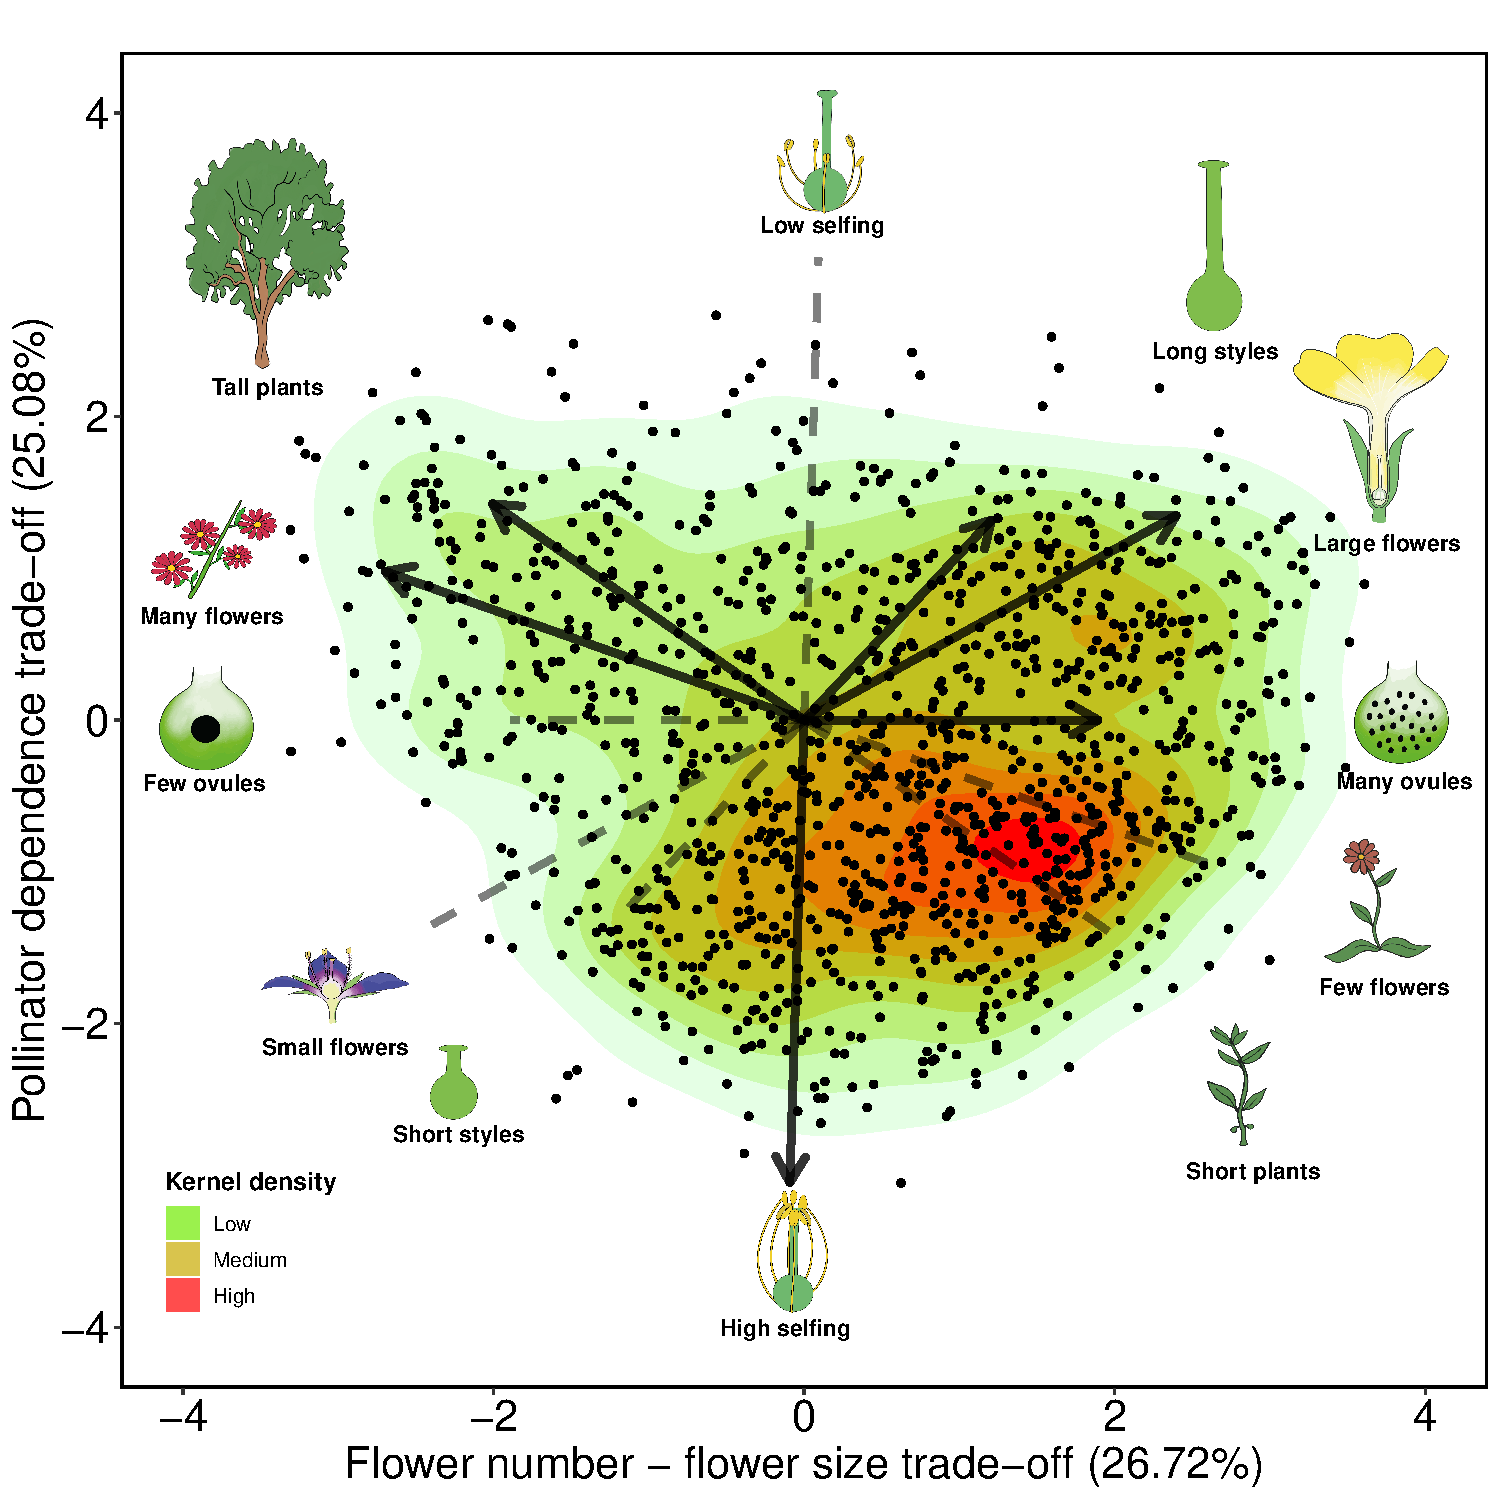
\includegraphics{output/figures/unnamed-chunk-1-1.pdf}
\caption{\label{fig:unnamed-chunk-1}Figure 1. Life history strategies for
1,236 plant species from 28 plant-pollinator networks studies across the
first two axes of trait variation from a phylogenetically informed
principal component analysis (pPCA). The solid arrows indicate the
direction of the different quantitative traits (flower number, plant
height, style length, flower size, ovule number and level of autonomous
selfing) in the 2-d plane. The length of the arrows indicate the weight
of the variables on each principal component and the labelled icons at
their end represent the extreme form of the trait continuum. The dashed
lines show the opposed direction of trait variation and the non-labelled
icons at their end illustrate the opposing extreme of the continuum.}
\end{figure}

We found that most categorical traits were statistically associated with
the first two axes of trait variation (Figure 2 and Table S2). Flower
symmetry, which was only associated with PC2 (Sum of squares = 8.51,
F-value = 14.72, p \textless{} 0.01 ), and nectar provision, which was
independent of PC1 and PC2 (PC1: Sum of squares = 0.37, F-value = 0.29 ,
p = 0.59; PC2: Sum of squares = 0.83, F-value = 1.43, p = 0.23) showed
lack of statistical association. In addition, we found statistical
differences (Tukey test) between the different levels of categorical
traits in the trait space (Figure S7). Regarding self compatibility, we
found larger differences on PC2 (i.e., species with unisexual flowers
that were self incompatibile were statistically differentiated from
species with partial or full self compatibility; Figure S7 A and B).
Life forms differed statistically across both axes of trait variation
and followed a gradient of larger life forms (trees and shrubs) with
higher pollinator dependence to smaller ones (herbs) with lower
pollinator dependence (Figure S7 C and D). Consequently, lifespan also
followed this gradient but perennial and short lived species only
differed statistically on PC2 (Figure S7 E and F). Species with
unisexual flowers (monoecious and dioecious) were clustered on both
extremes of the first two principal components and had the highest
pollinator dependence and highest number of flowers (Figure S7 G and H).
Moreover, we found that the campanulate and capitulum flower shapes were
differentiated from tube, papilionaceous, open and brush shapes in the
trait space. The former morphologies had larger flowers and greater
pollinator dependence, while the latter had higher flower number and
greater autonomous selfing (Figure S7 I and J). Regarding flower
symmetry, zygomorphic flowers were associated with lower levels of
pollinator dependence, whereas actinomorphic flowers had higher levels
of pollinator dependence (Figure S7 K and L).

\blandscape

\begin{figure}[H]
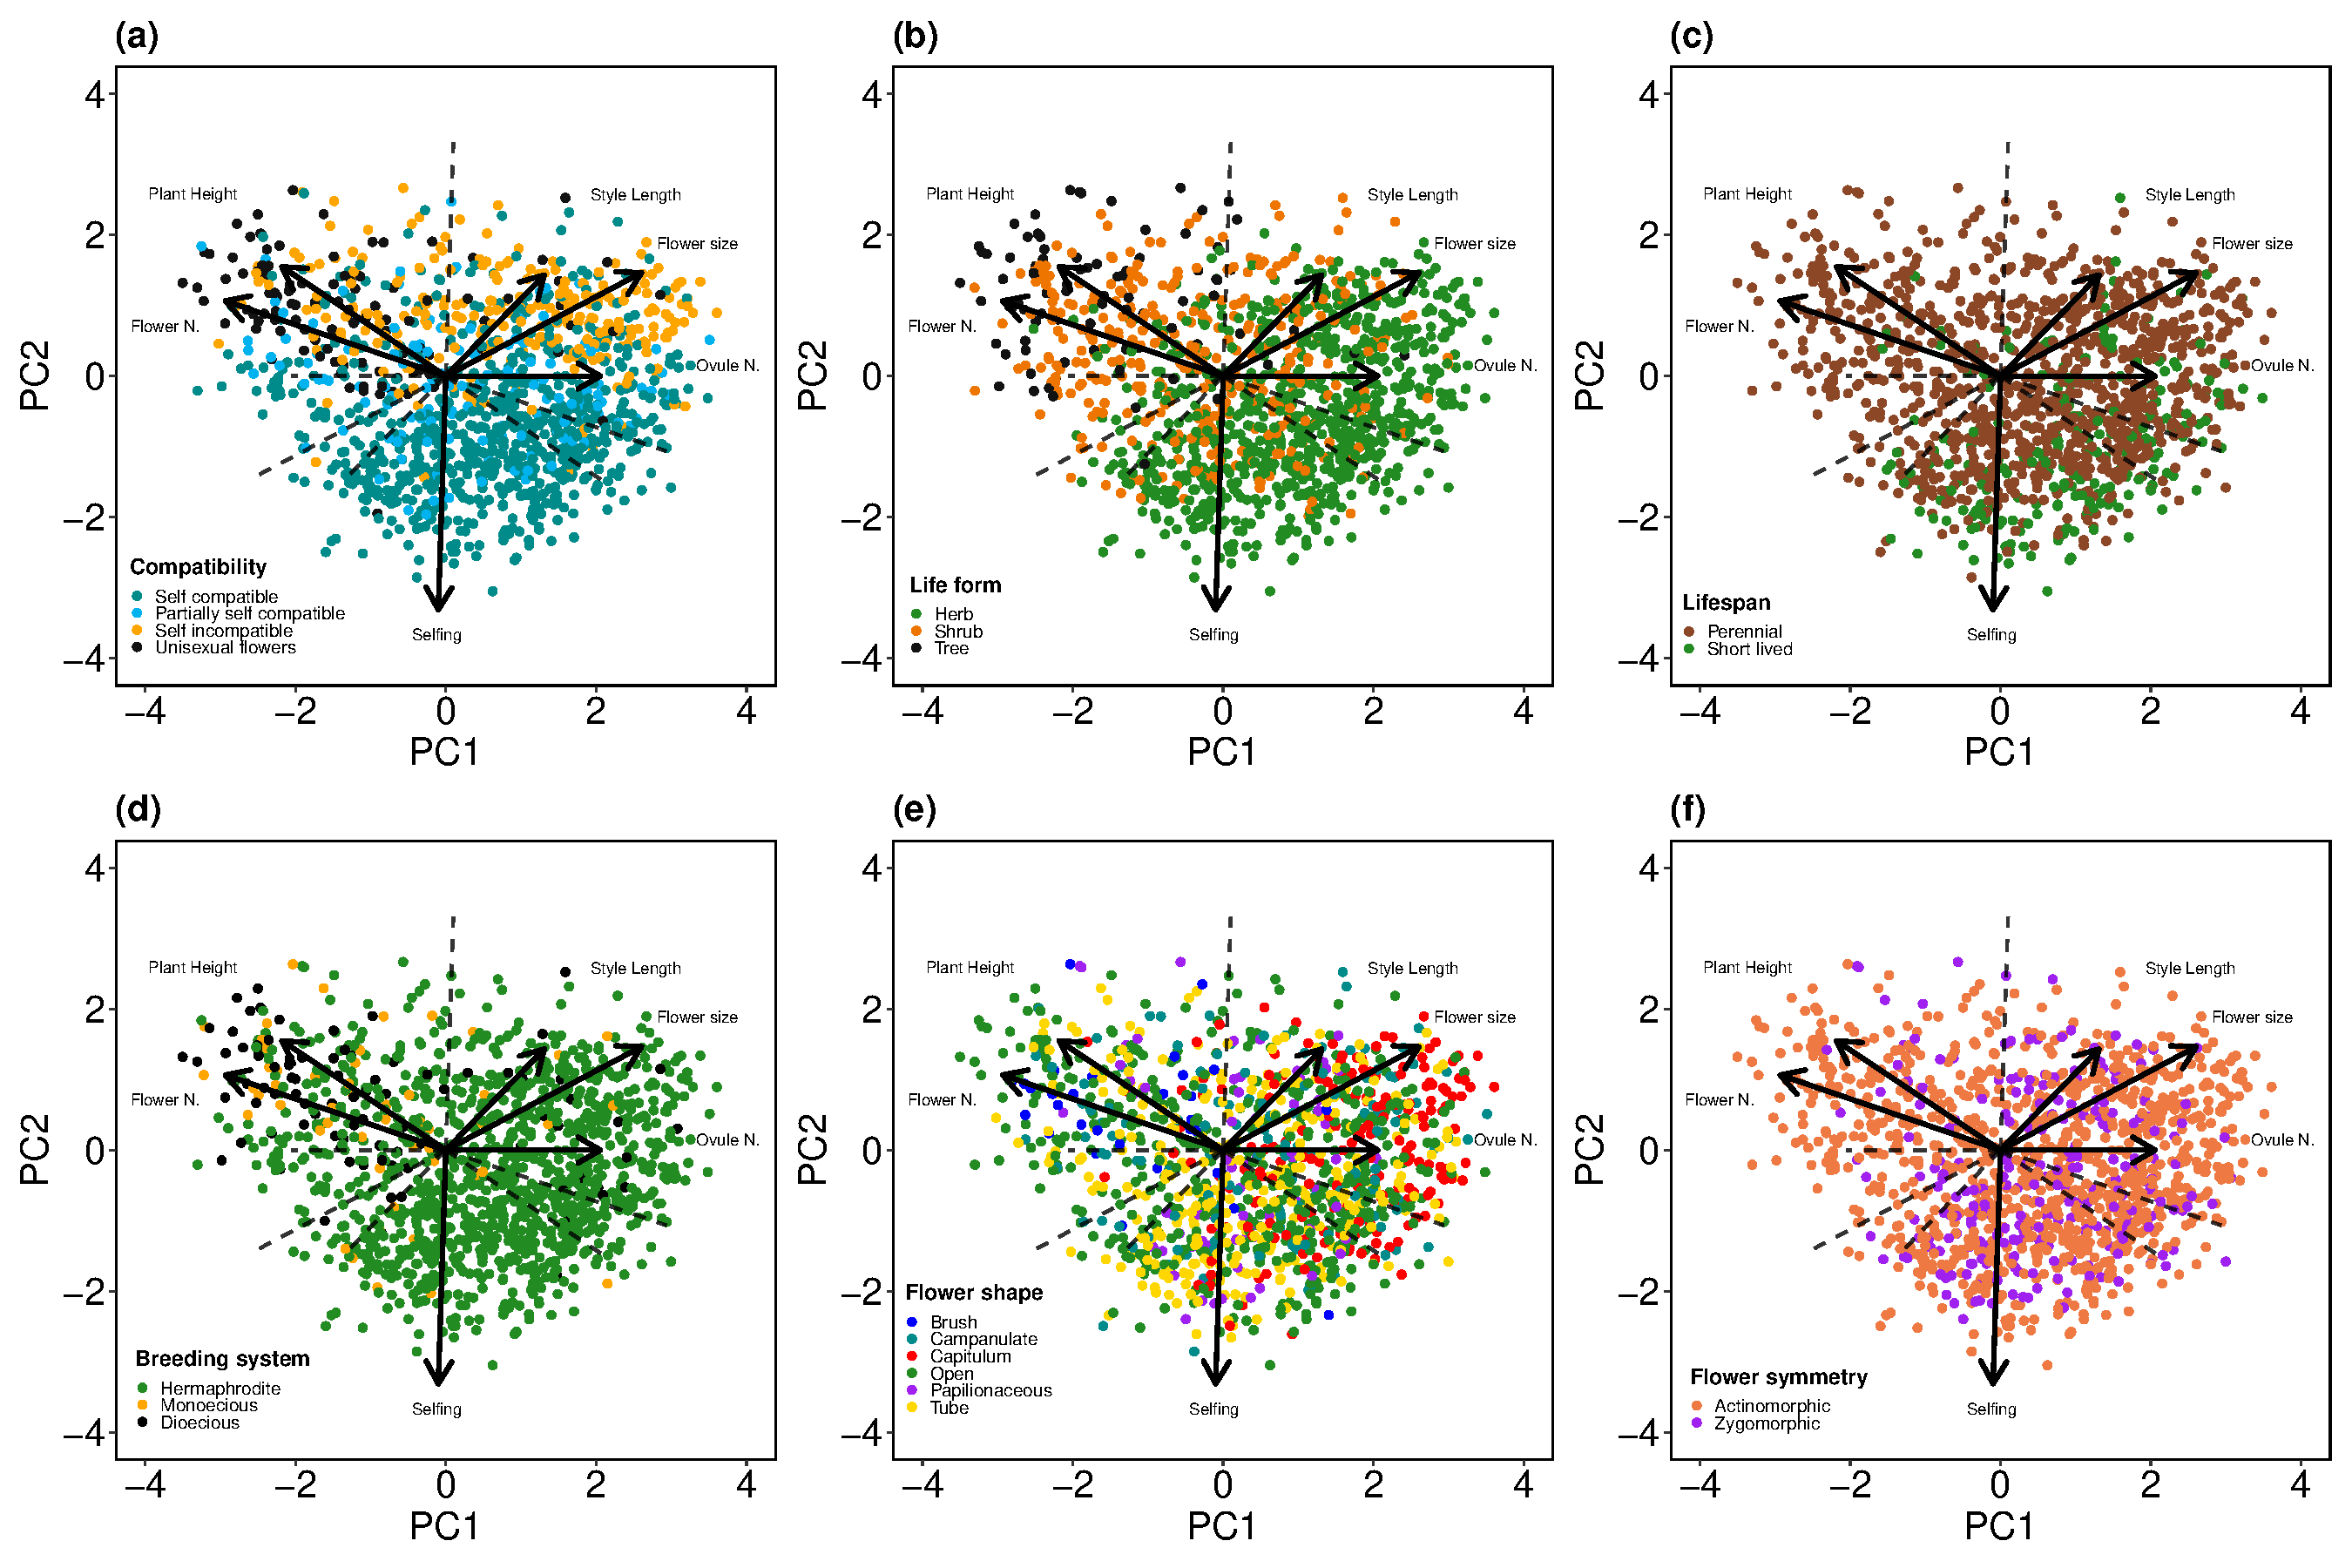
\includegraphics{output/figures/unnamed-chunk-2-1} \caption{Location of the different qualitative traits that showed statistical association with the first two axes of trait variation. These different traits included: compatibility system (a), life form (b), lifespan (c), breeding system (d), flower shape (e) and flower symmetry (f).}\label{fig:unnamed-chunk-2}
\end{figure}

\elandscape

\textbf{Phylogenetic signal of traits}

\subsubsection{OLD}\label{old}

Among flowering plants there is an astonishing diversity of floral
structures and plant reproductive strategies (Barrett
\protect\hyperlink{ref-barrett2002}{2002}, Schiestl and Johnson
\protect\hyperlink{ref-schiestl2013}{2013}). Subsequently, pollination
biologists have long studied their relevance on plant-pollinator
interactions. However, despite recent efforts exploring reproductive
(e.g., mating and compatibility system) and floral traits (e.g., flower
size or nectar provision) with large sets of species (Carvalheiro et al.
\protect\hyperlink{ref-carvalheiro2014}{2014}, Baude et al.
\protect\hyperlink{ref-baude2016}{2016}, Munoz et al.
\protect\hyperlink{ref-munoz2016}{2016}, Grossenbacher et al.
\protect\hyperlink{ref-grossenbacher2017}{2017}, Moeller et al.
\protect\hyperlink{ref-moeller2017}{2017}), most studies focus on the
individual, community level or specific taxa and macroecological
patterns remain poorly investigated. For instance, studies depicting
species' life history strategies generally focus on vegetative traits
and rarely consider reproductive traits on the main axes of trait
variation (Díaz et al. \protect\hyperlink{ref-diaz2016}{2016},
Salguero-Gómez et al. \protect\hyperlink{ref-salguero2016}{2016}). In
addition, there is not a unified framework that explores the compromises
of floral traits and their relevance on plant life strategies (Roddy et
al. \protect\hyperlink{ref-roddy2021}{2021}). Similarly, there is
growing interest in understanding what determines plant-pollinator
network structure. Approaches with traits range from the description of
pollination syndromes (e.g., Dellinger
\protect\hyperlink{ref-dellinger2020}{2020}), to more specific
trait-matching analysis (Bartomeus et al.
\protect\hyperlink{ref-bartomeus2016}{2016}), but again the reproductive
biology of the species has received little attention (but see Tur et al.
\protect\hyperlink{ref-tur2013}{2013} and @devaux2014) and floral traits
have been overlooked beyond highly specialised plant-pollinator
interactions (Dellinger \protect\hyperlink{ref-dellinger2020}{2020},
Roddy et al. \protect\hyperlink{ref-roddy2021}{2021}).

With increased availability of large trait databases, plant ecological
strategies have begun to be examined more frequently (e.g., TRY, Kattge
et al. \protect\hyperlink{ref-kattge2011}{2011} and COMPADRE,
Salguero-Gómez et al. \protect\hyperlink{ref-salguero2015}{2015}),
highlighting global patterns and constraints of plant form and function
(Díaz et al. \protect\hyperlink{ref-diaz2016}{2016}, Salguero-Gómez et
al. \protect\hyperlink{ref-salguero2016}{2016}, Carmona et al.
\protect\hyperlink{ref-carmona2021}{2021}). However, these resources and
their research have mainly focused on vegetative traits such as the leaf
(Wright et al. \protect\hyperlink{ref-wright2004}{2004}) or wood (Chave
et al. \protect\hyperlink{ref-chave2009}{2009}) trade-offs and neglected
reproductive and floral traits that also can influence the spectrum of
trait variation. For instance, short lived and perennial species tend to
have high and low levels of outcrossing respectively (Barrett
\protect\hyperlink{ref-barrett2003}{2003}, Moeller et al.
\protect\hyperlink{ref-moeller2017}{2017}) and outcrossing levels have
been shown to be positively correlated with flower size (Goodwillie et
al. \protect\hyperlink{ref-goodwillie2010}{2010}). In addition, the
presence of costly rewards (e.g., pollen or nectar) and showy flowers or
floral displays cannot be understood without considering pollinators
that are thought to be responsible for approximately 87.5\% of the
pollination of flowering plants (Ollerton et al.
\protect\hyperlink{ref-ollerton2011}{2011}). Hence, exploring plant life
strategies with reproductive and floral trade-offs, in conjunction with
their known pollinators seems necessary for a correct understanding of
the plant economics.

Several key studies have progressed knowledge of the link between traits
and network properties (Lázaro et al.
\protect\hyperlink{ref-lazaro2008}{2008}, Bartomeus
\protect\hyperlink{ref-bartomeus2013}{2013}, Carvalheiro et al.
\protect\hyperlink{ref-carvalheiro2014}{2014}, Klumpers et al.
\protect\hyperlink{ref-klumpers2019}{2019}). Functional traits can
determine whether species interact, and thus define the species network
role (e.g., specialist vs generalist). For instance, species with high
investment in floral display tend to have higher visitation rates (Stang
et al. \protect\hyperlink{ref-stang2006}{2006}, Novella-Fernandez et al.
\protect\hyperlink{ref-novella-fernandez2019}{2019}) and greater
specialization is generally associated with occupation of the trait
space extremes (Junker et al. \protect\hyperlink{ref-junker2013}{2013},
Coux et al. \protect\hyperlink{ref-coux2016}{2016}). In addition, the
structure of the pollination network highly depends on the degree of
trait-matching between plants and pollinators (Stang et al.
\protect\hyperlink{ref-stang2009}{2009}, Ibanez
\protect\hyperlink{ref-ibanez2012}{2012}, Peralta et al.
\protect\hyperlink{ref-peralta2020}{2020}). However, little is known
about the consequences of reproductive traits and floral rewards on
plant species roles. In addition, although some attempts have been made
to evaluate trait relationships in plant-pollinator interactions at a
global scale (Carvalheiro et al.
\protect\hyperlink{ref-carvalheiro2014}{2014}, Rech et al.
\protect\hyperlink{ref-rech2016}{2016}), macroecological patterns have
been little explored.

Here, we explore the major axes of plant reproductive trait variation.
We investigate how these traits influence the structure of
plant-pollinator networks by compiling a unique dataset comprising 20
plant functional traits for 1,506 species from 64 unique networks and 8
metawebs. First, we evaluate the major axes of reproductive trait
variation and tradeoffs that determine plant form and function. Second,
we investigate how plant species' position in trait-space influences
interaction strength with different pollinator functional groups.
Finally, we assess the relevance of the main axes of trait variation and
traits in understanding the plant species role within the networks with
complementary species level metrics (i.e., interaction strength,
normalized degree and specialization).

\section{METHODS}\label{methods}

\subsection{Plant-pollinator network
studies}\label{plant-pollinator-network-studies}

We selected 28 studies from 18 different countries that constituted a
total of 64 plant-pollinator networks. All these studies censored
plant-pollinator interactions in natural systems and were selected in
order to have a wide representation of geographical areas of the world.
Although these studies differ in sampling effort and methodology, all
studies provided information about plant-pollinator interactions
(weighted and non-weighted) allowing us to build a database of plants
that are likely to be animal pollinated. Some of these networks have
been already used in past studies of plant-pollinator networks (Olesen
et al. \protect\hyperlink{ref-olesen2007}{2007}, Fortuna et al.
\protect\hyperlink{ref-fortuna2010}{2010}, Carvalheiro et al.
\protect\hyperlink{ref-carvalheiro2014}{2014}) and are available on the
online networks archives The Web of Life (Fortuna et al.
\protect\hyperlink{ref-fortuna2014}{2014}) and Mangal (Poisot et al.
\protect\hyperlink{ref-poisot2016}{2016}). In total, our network dataset
(Table S1) constituted 60 weighted (interaction frequency) and 4 binary
networks, each sampled at a unique location and year, as well as 8
meta-webs where sampled interactions were pooled across several
locations and multiple years.

\subsection{Taxonomy of plants and
pollinators}\label{taxonomy-of-plants-and-pollinators}

All plant species names, genera, families and orders were retrieved and
standardized from the taxonomy data sources NCBI
(\url{https://www.ncbi.nlm.nih.gov/taxonomy}) (plants) and ITIS
(\url{https://www.itis.gov/}) (pollinators) using the R package taxize
(version 0.9.99, Chamberlain et al.
\protect\hyperlink{ref-chamberlain2020}{2020}). We filled the `not
found' searches manually using \url{http://www.theplantlist.org/} and
\url{http://www.mobot.org/} for plants and
\url{http://www.catalogueoflife.org/} for floral visitors.

\subsection{Functional traits}\label{functional-traits}

We selected 20 different functional traits based on their relevance to
plant reproduction and data availability (Table 1). The selected traits
were quantitative (12) and categorical (8) and belonged to three
different trait types: vegetative, floral and reproductive. For each
species, we undertook an extensive literature and online search across a
wide range of resources (plant databases, online floras, books, journals
and images) from a total of 30,120 cells (20 columns x 1,506 spp) we
were able to fill 23,969 cells (79.6\% of the dataset, see Figure S1 for
missing values information per variable).

\setstretch{1.25}

\begin{table}

\caption{\label{tab:unnamed-chunk-3}List of the 20 traits compiled in this study divided in quantitative and categorical traits. The different types of trait (vegetative ‘V’, floral ‘F’ and reproductive ‘R’), total records found for the 1,506 species and categories of the qualitative traits are also provided. }
\centering
\fontsize{10}{12}\selectfont
\begin{tabu} to \linewidth {>{}c>{\raggedright}X>{\centering}X>{}c>{\raggedright}X>{\raggedright}X>{\centering}X}
\toprule
\multicolumn{3}{c}{\textbf{Quantitative traits}} & \multicolumn{4}{c}{\textbf{Categorical traits}} \\
\cmidrule(l{3pt}r{3pt}){1-3} \cmidrule(l{3pt}r{3pt}){4-7}
\textbf{Type} & \textbf{Traits} & \textbf{Records} & \textbf{Type} & \textbf{Traits} & \textbf{Categories} & \textbf{Records}\\
\midrule
\textbf{V} & Plant height (m) & 1470 & \textbf{V} & Lifepan & \makecell[l]{Short-lived \\ Perennial} & 1466\\
\addlinespace
\textbf{F} & Flower width (mm) & 1472 & \textbf{V} & Life form & \makecell[l]{Herb \\ Shrub \\ Tree} & 1472\\
\addlinespace
\textbf{F} & Flower length (mm) & 1401 & \textbf{F} & Flower shape & \makecell[l]{Brush \\ Campanulate \\ Capitulum \\ Open \\ Papilionaceous \\ Tube} & 1458\\
\addlinespace
\textbf{F} & Inflorescence width (mm) & 1496 & \textbf{F} & Flower symmetry & \makecell[l]{Actinomorphic \\ Zygomorphic} & 1478\\
\addlinespace
\textbf{F} & Style length (mm) & 1497 & \textbf{F} & Nectar & \makecell[l]{Presence \\ Absence} & 1408\\
\addlinespace
\textbf{F} & Ovules per flower & 1457 & \textbf{R} & Autonomous selfing & \makecell[l]{None \\ Low \\ Medium \\ High} & 987\\
\addlinespace
\textbf{F} & Flowers per plant & 1468 & \textbf{R} & Compatibility system & \makecell[l]{Self-incomp. \\ Partially self-comp. \\ Self-comp.} & 1253\\
\addlinespace
\textbf{F} & Nectar ($\mu$l) & 531 & \textbf{R} & Breeding system & \makecell[l]{Hermaphrodite \\ Monoecious \\ Dioecious} & 1489\\
\addlinespace
\textbf{F} & Nectar (mg) & 455 & \textbf{} &  &  & \\
\addlinespace
\textbf{F} & Nectar concentration ($\%$) & 558 & \textbf{} &  &  & \\
\addlinespace
\textbf{F} & Pollen grains per flower & 533 & \textbf{} &  &  & \\
\addlinespace
\textbf{R} & Autonomous selfing (fruit set) & 992 & \textbf{} &  &  & \\
\bottomrule
\end{tabu}
\end{table}

\setstretch{2}

\subsection{Phylogenetic Distance}\label{phylogenetic-distance}

We calculated the phylogenetic distance between different plant species
using the function get\_tree from the package rtrees (downloaded from
github, \url{https://github.com/daijiang/rtrees}), which downloads
phylogenetic distances from the extended R implementation of the Open
Tree of Life (Smith and Brown \protect\hyperlink{ref-smith2018}{2018})
developed by Jin and Qian (\protect\hyperlink{ref-jin2019}{2019}).

\subsection{Data Imputation}\label{data-imputation}

Missing values were imputed with the function missForest (Stekhoven and
Bühlmann \protect\hyperlink{ref-stekhoven2012}{2012}) which allows
imputation of data sets with continuous and categorical variables. We
accounted for the phylogenetic distance among species on the imputation
process by including the eigenvectors of a principal component analysis
of the phylogenetic distance (PCoA) which has been shown to improve the
performance of missForest (Penone et al.
\protect\hyperlink{ref-penone2014}{2014}). To extract the eigenvectors,
we used the function PVRdecomp from the package PVR (Santos et al.
\protect\hyperlink{ref-santos2018}{2018}) based on the conceptual
framework of Diniz-Filho et al.
(\protect\hyperlink{ref-diniz-filho2012}{2012}). Although the variable
of autonomous selfing had a high percentage of missing values (68\%), we
were able to solve this by back transforming the qualitative column of
autonomous selfing to numerical. The categories of `none', `low',
`medium' and `high' were converted to representative percentages of each
category 0\%, 13\%, 50.8\% and 80\% respectively. This reduced the
percentage of missing values for this column from 68\% to 35\% and
allowed the imputation of this variable. However, we were unable to
impute nectar and pollen quantity due to the high percentage of missing
values (Figure S1). The imputed dataset had 9.7\% of missing values with
a total of 8 categorical and 8 numerical variables. Finally, we
conducted an additional imputation for the subset of species with
quantitative information of nectar and pollen; all variables had lower
than 30\% of missing values (N = 636) and the total proportion of
missing values in this dataset considering all variables was 13\%.

\subsection{Plant strategies}\label{plant-strategies}

We explored the trade-offs between different quantitative plant
functional traits with a phylogenetically informed Principal Component
Analysis (pPCA). We did not include the quantitative variables of flower
length and inflorescence width because they were highly and moderately
correlated to flower width (Pearson's correlation = 0.72, p \textless{}
0.01 and Pearson's correlation = 0.36, p \textless{} 0.01 respectively),
and thus we avoided overemphasizing flower size on the spectrum of trait
variation. In addition, we explored the location of different
qualitative traits in the trait space. Prior to the analyses, we
excluded outliers and standardized the data. Due to the high sensitivity
of dimensionality reduction to outliers, we excluded values in the
2.5th-97.5th percentile range (Legendre and Legendre
\protect\hyperlink{ref-legendre2012}{2012}). Then, we log transformed
the variables to reduce the influence of outliers and z-transformed (X=
0, SD=1) so that all variables were within the same numerical range. We
performed the pPCA using the function phyl.pca from the package phytools
(version number 0.7-70, Revell \protect\hyperlink{ref-revell2012}{2012})
with the method lambda (\(\lambda\)) that calculates the phylogenetic
correlation between 0 (phylogenetic independence) and 1 (shared
evolutionary history) and we implemented the mode covariance because our
variables are on the same scale after the log and z-transformation (Abdi
and Williams \protect\hyperlink{ref-abdi2010}{2010}). Moreover, to
corroborate that our imputation of missing values did not affect our
results, we conducted a pPCA on the full dataset without missing values
(Figure S2). We found little difference between the variance explained
with the imputed dataset (51.08\%) and the dataset without missing
values (56.26\%). In addition, the loadings on each principal component
had a similar contribution and correlation patterns, with the exception
of plant height which showed slight variations between the imputed and
non imputed dataset. Finally, we explored with the imputed dataset with
quantitative information of pollen and nectar the compromises in the
trait space of these two floral rewards with the other quantitative
traits. For this, we considered solely one variable of nectar quantity
(microlites of nectar per flower) in order to avoid overemphasizing
nectar on the spectrum of trait variation.

\subsection{Phylogenetic signal of
traits}\label{phylogenetic-signal-of-traits}

We calculated the phylogenetic signal of the different quantitative
traits on the imputed dataset with the full set of species (N = 1506)
with the package phytools version 0.7-70 (Revell
\protect\hyperlink{ref-revell2012}{2012}) and we used Pagel's lambda
(\(\lambda\)) as a measurement of the phylogenetic signal. For pollen
and nectar traits, phylogenetic signal was calculated on the imputed
dataset that included these traits (N = 636).

\subsection{Networks analysis}\label{networks-analysis}

Our analyses were conducted on the subset of 60 weighted networks with
interaction frequency sampled in a unique flowering season and site.
Although floral visitors are not always pollinators and the frequency of
visits does not consider each pollinator species efficiency (Ballantyne
et al. \protect\hyperlink{ref-ballantyne2015}{2015}), interaction
frequency provides valuable information of the impact of pollinators
(Vázquez et al., 2005; Vázquez et al., 2012). Although not all networks
were sampled using the same method, our aim was not to compare patterns
across networks but within each network in order to obtain a general
picture of associations between traits and the main axes of trait
variation and plant species functional roles.

\emph{Functional groups visitation patterns}

We explored the relevance of pollinator functional groups and the main
axes of trait variation (pPCA with imputed dataset) on pollinator
visitation per plant species. For this, we divided floral visitors into
six main groups that differ in life form and behaviour: (i)
Hymenoptera-Anthophila (bees), (ii) Hymenoptera-non-Anthophila (other
non-bee Hymenoptera), (iii) Diptera-Syrphids, (iv) Diptera-Non-Syrphids,
(v) Lepidoptera and (vi) Coleoptera. In addition, because Hymenoptera
was the most represented group with 2,256 records counted and had the
highest frequency of visits of all groups, we also explored visitation
patterns of the most represented families of Hymenoptera on the trait
space (Andrenidae, Apidae, Colletidae, Halictidae and Megachilidae).
Apis mellifera was the species with the largest proportion of records
(7.55\% from the total) which is is consistent with the results of Hung
et al. (\protect\hyperlink{ref-hung2018}{2018}) that showed that A.
mellifera was the most frequent visiting species on a similar dataset of
80 interaction plant-pollinator networks on natural systems. Hence, to
control for the relevance of Apis mellifera on the observed visitation
patterns of bees, we conducted an analogous analysis excluding A.
mellifera. We found that A. mellifera, was driving, in part, some of the
observed trends on PC1 (Figure S3). However, we did not find major
changes on PC2 and PC3.

\emph{Plant species functional roles}

We investigated if the main axes of trait variation and traits explained
plant species functional roles. We considered all uncorrelated traits
apart from the principal components because this allowed us to consider
quantitative and categorical traits. For this, we also used a modelling
approach and conducted decision trees which help to interpret visually
how the different traits determine species functional roles. We selected
simple and complementary plant species level metrics with a relatively
straightforward ecological interpretation relevant to our research
goals: (i) sum of visits per plant species; (ii) normalized degree
calculated as the number of links per plant species divided by the
possible number of partners which helps comparison across networks; and
(iii) specialization (d') (Blüthgen et al.
\protect\hyperlink{ref-bluthgen2006}{2006}), which measures the
deviation of an expected random choice of the available interaction
partners and ranges between 0 (maximum generalization) and 1 (maximum
specialization). Normalized degree and specialization were calculated
with the specieslevel function from the R package bipartite (version
2.15, Dormann et al. \protect\hyperlink{ref-dormann2008}{2008}).

\subsection{Analyses}\label{analyses}

First, we implemented Bayesian generalized linear mixed models using the
R package brms (version 2.14.6, Bürkner
\protect\hyperlink{ref-burkner2017}{2017}). We modelled the frequency of
visits as a function of the main axes of trait variation and floral
visitors functional groups
(Visits\textasciitilde{}PC1xFG+PC2xFG+PC3xFG). Because we were
interested in possible differences among main visitor guilds to plants
with different strategies, we included the interaction between the main
axes of trait variation and the distinct floral visitor functional
groups. We added a nested random effect with networks nested on the
study system to capture the network variability per study and within
networks. We specified this model with a zero inflated negative binomial
distribution and weakly informative priors from the brms function.
Moreover, we included the phylogenetic covariance matrix as a random
factor due to the possible shared evolutionary history of the species
and therefore lack of independence across them.

Second, we modelled the distinct plant species metrics (sum of visits,
normalized degree and plant specialization) as a function of the three
main axes of trait variation in three different models for each metric
(plant species level metric\textasciitilde{}PC1+PC2+PC3). In addition we
also explored how all uncorrelated traits (13) explained these metrics
in three other models (plant species level metric \textasciitilde{}
plant height + lifespan + life form + flower shape + flower symmetry +
flower width + style length + ovule number + flowers per plant + nectar
provision + autonomous selfing + compatibility system + breeding
system). For each response variable (metric), we used different
distribution families: zero inflated negative binomial for the sum of
visits, weibull for normalized degree and zero one inflated beta for
specialization. Moreover, we included a nested random effect with
networks nested on the study system and a phylogenetic random effect for
species (as detailed above) in each model.

All analyses were conducted in R Version 4.0.3. In addition, all models
were run for 3,000 iterations with 1000 warm up iterations. We set delta
() to 0.99 to avoid divergent transitions and visualized the posterior
predictive checks with the function pp\_check using the bayesplot
package (version 1.7.2, Gabry et al., 2019).

{[}ADD REGRESSION TREE TO METHODS{]} We conducted regression trees in
order to explore the relevance of traits on the species plant functional
role. We repeated the procedure as the modelling analysis and we ran a
decision tree for each plant level species metric (interaction
frequency, normalized degree and specialization). We used the full
datase

rpart 4.1-15 (Therneau et al., 2019) rpart.plot 3.0.9 (Milborrow 2018)

\section{RESULTS}\label{results-1}

\subsection{Plant strategies}\label{plant-strategies-1}

The phylogenetically informed principal component analysis (pPCA)
captured with the first two and three axes 51.8\% and 70.97\% of the
trait variation respectively (Figure 1 and Figure S4) and had a
phylogenetic correlation (\(\lambda\)) of 0.76. The first principal
component (PC1) represented 26.72\% of the trait variation and showed
the flower number versus flower size compromise. Thus, as flower number
and plant height increase, flower size, style length and ovule number
decrease; and, as flower size, style length and ovule number increase,
flower number and plant height decrease. The main contributing traits to
PC1 were plant height, flower number, ovule number and flower size
(loadings \textgreater{} \textbar{}0.5\textbar{}; Table S2) but style
length also contributed moderately on PC1 (loading = -0.33). The second
principal component (PC2) represented 25.05\% of the trait variation and
showed the trade-off between low and high pollinator dependence and we
refer to this axis as the pollinator dependence trade-off. The main
driver of trait variation of PC2 was autonomous selfing (loading = 0.85)
but the other traits (except ovule number) also made a moderate
contribution to PC2 (loadings from 0.27 to 0.4; Table S2). We found that
high pollinator dependence was associated with larger and higher number
of flowers, greater plant height and longer styles. In contrast, species
with high levels of autonomous selfing had a general lower investment in
flower number and size, plant height and style length. Further, PC3 also
explained a considerable amount of variability (19.17\%) and the main
contributors to this axis were style length (loading = -0.66) and the
degree of autonomous selfing (loading = -0.51). The remaining traits,
apart from ovule number, were moderately correlated to changes on PC3
(loadings from -0.23 to -0.46; Table S2). In addition, the pPCA with the
species subset that had nectar and pollen quantity showed that nectar
quantity (microlitres of nectar per flower) was positively associated
with flower size, style length and ovule number (PC1, 24.70\%); and
pollen quantity was positively correlated with flower number and plant
height and negatively associated with autonomous selfing (PC2, 20.59\%;
Figure S5). This pPCA also showed similar explained variance with two
components (50.06\%) and similar associations of traits despite some
variability in the loadings (Table S3).

\begin{figure}
\centering
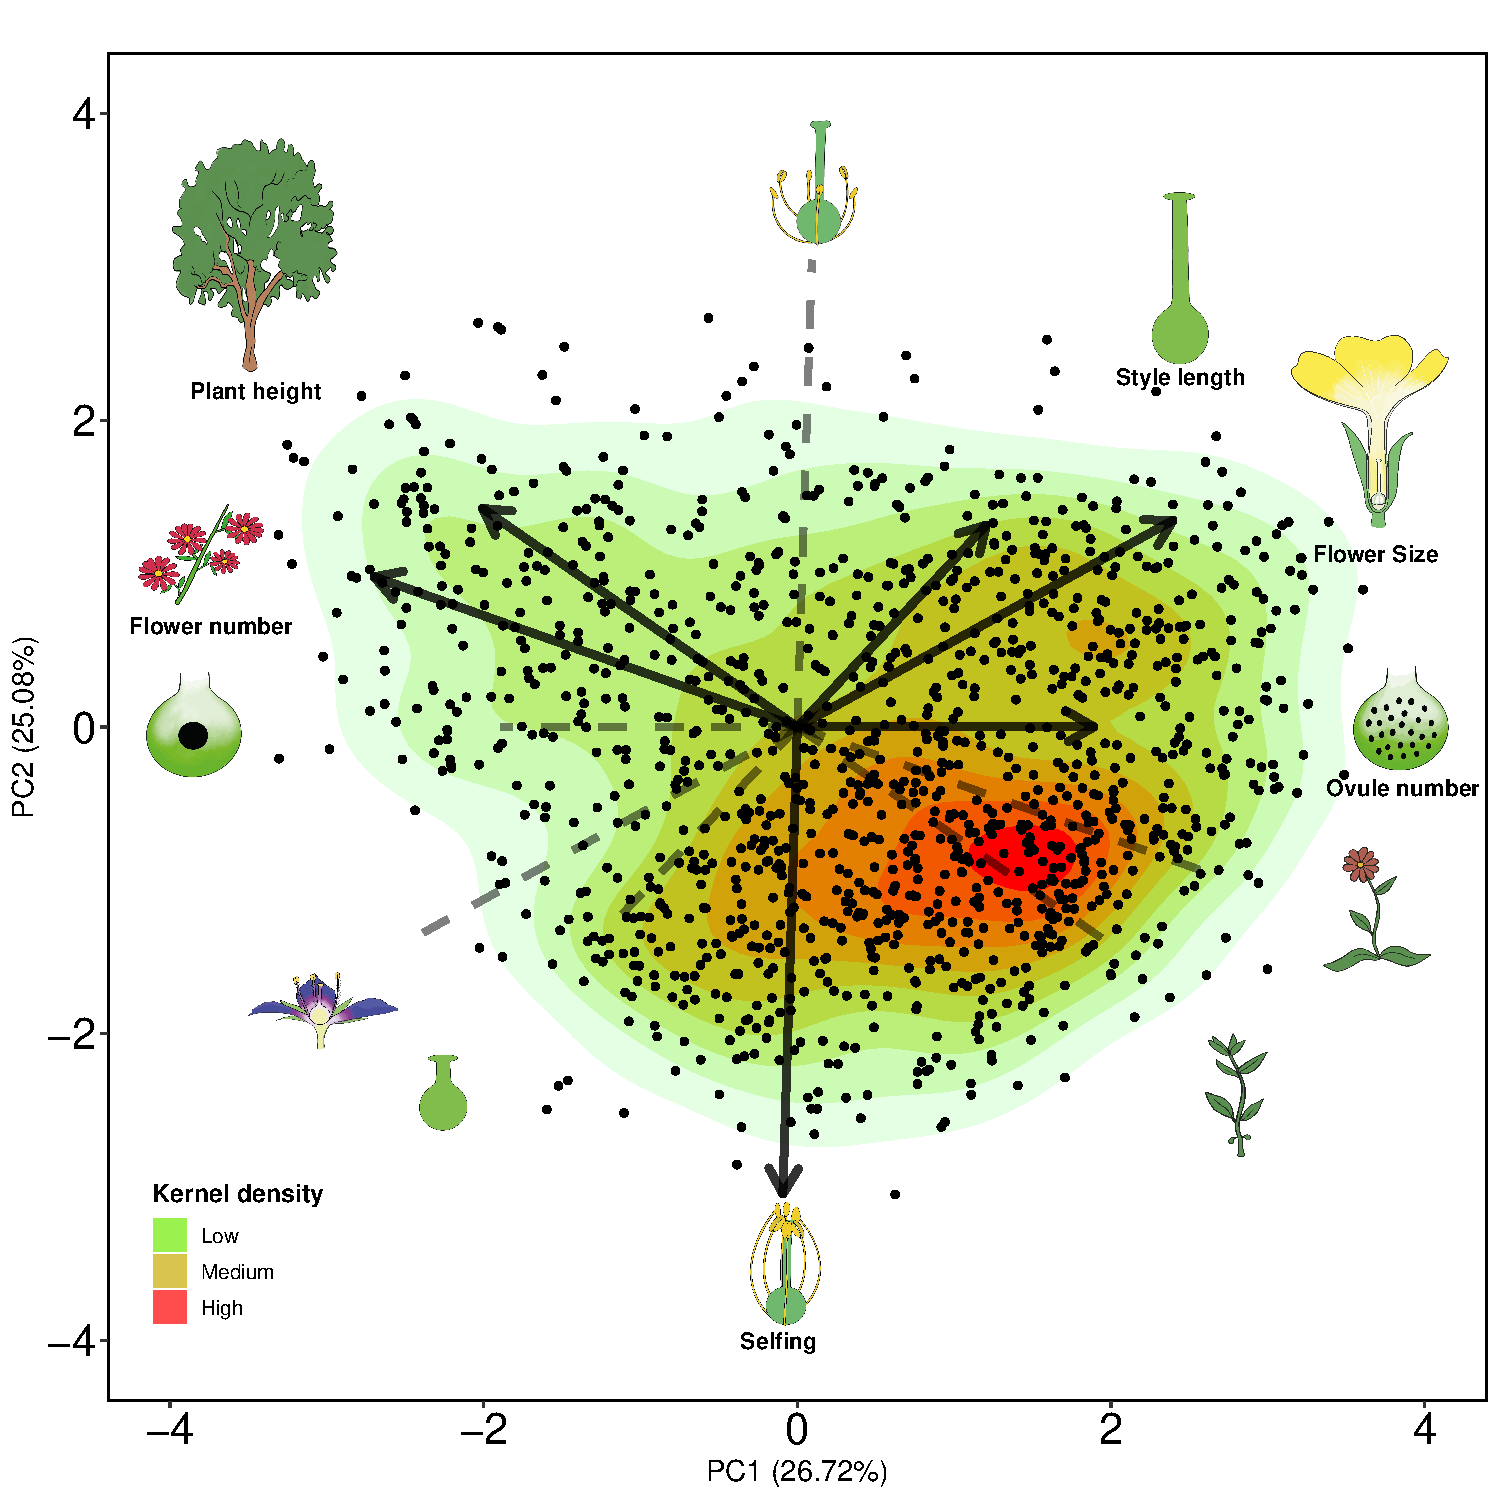
\includegraphics{output/figures/unnamed-chunk-4-1.pdf}
\caption{\label{fig:unnamed-chunk-4}Life history strategies for 1,236 plant
species from 29 plant-pollinator networks studies across the first two
axes of variation from a phylogenetically informed principal component
analysis (pPCA). The solid arrows indicate the direction and weights of
the six quantitative traits (flower number, plant height, style length,
flower size, ovule number and autonomous selfing level) and the labelled
icons at their end represent the extreme form of the trait continuum.
The dashed lines indicate the opposed direction of trait variation and
the non-labelled icons at their end illustrate the other extreme of the
continuum.}
\end{figure}

Evaluation of qualitative variable positions in the trait space revealed
statistical association on both axes of trait variation for
compatibility, breeding system, life form, lifespan and flower shape
(Figure 2 and Table S4). In addition, flower symmetry was associated
with PC2 (Sum of squares = 8.51, F-value = 14.72 , p \textless{} 0.01 ).
Nectar provision was independent of both axes (PC1 Sum of squares =
0.37, F-value = 0.29 , p = 0.59; PC2 Sum of squares = 0.83, F-value =
1.43 , p = 0.23). Concerning self compatibility, we found larger
differences in pollinator dependence the trade off (i.e., species with
unisexual flowers and self incompatibility were statistically
differentiated from species with partially and fullyself compatibility
in trait space; Figure S3 A and B). Life forms differed statistically
across both axes of trait variation and followed a gradient of larger
life forms (trees and shrubs) with higher pollinator dependence to
smaller ones (herbs) with lower pollinator dependence (Figure S3 C and
D). Consequently, lifespan also followed this gradient but perennial and
short lived species just differed statistically on PC2 (Figure S3 E and
F). Species with unisexual flowers (monoecious and dioecious) were
clustered on both extremes of trait variation with the highest
pollinator dependence and flower number investment (Figure S3 G and H).
Moreover, we found that the campanulate and capitulum flower shapes were
differentiated from tube, papilionaceous, open and brush shapes in the
trait space. The former morphologies tended to occupy positions with
larger flowers and greater pollination dependence, while the latter
positions had higher number of flowers and autonomous selfing (Figure S3
I and J). Regarding flower symmetry, zygomorphic flowers were associated
with lower levels of pollinator dependence, whereas actinomorphic
flowers had higher pollinator dependence (Figure S3 K and L).

\begin{figure}
\centering
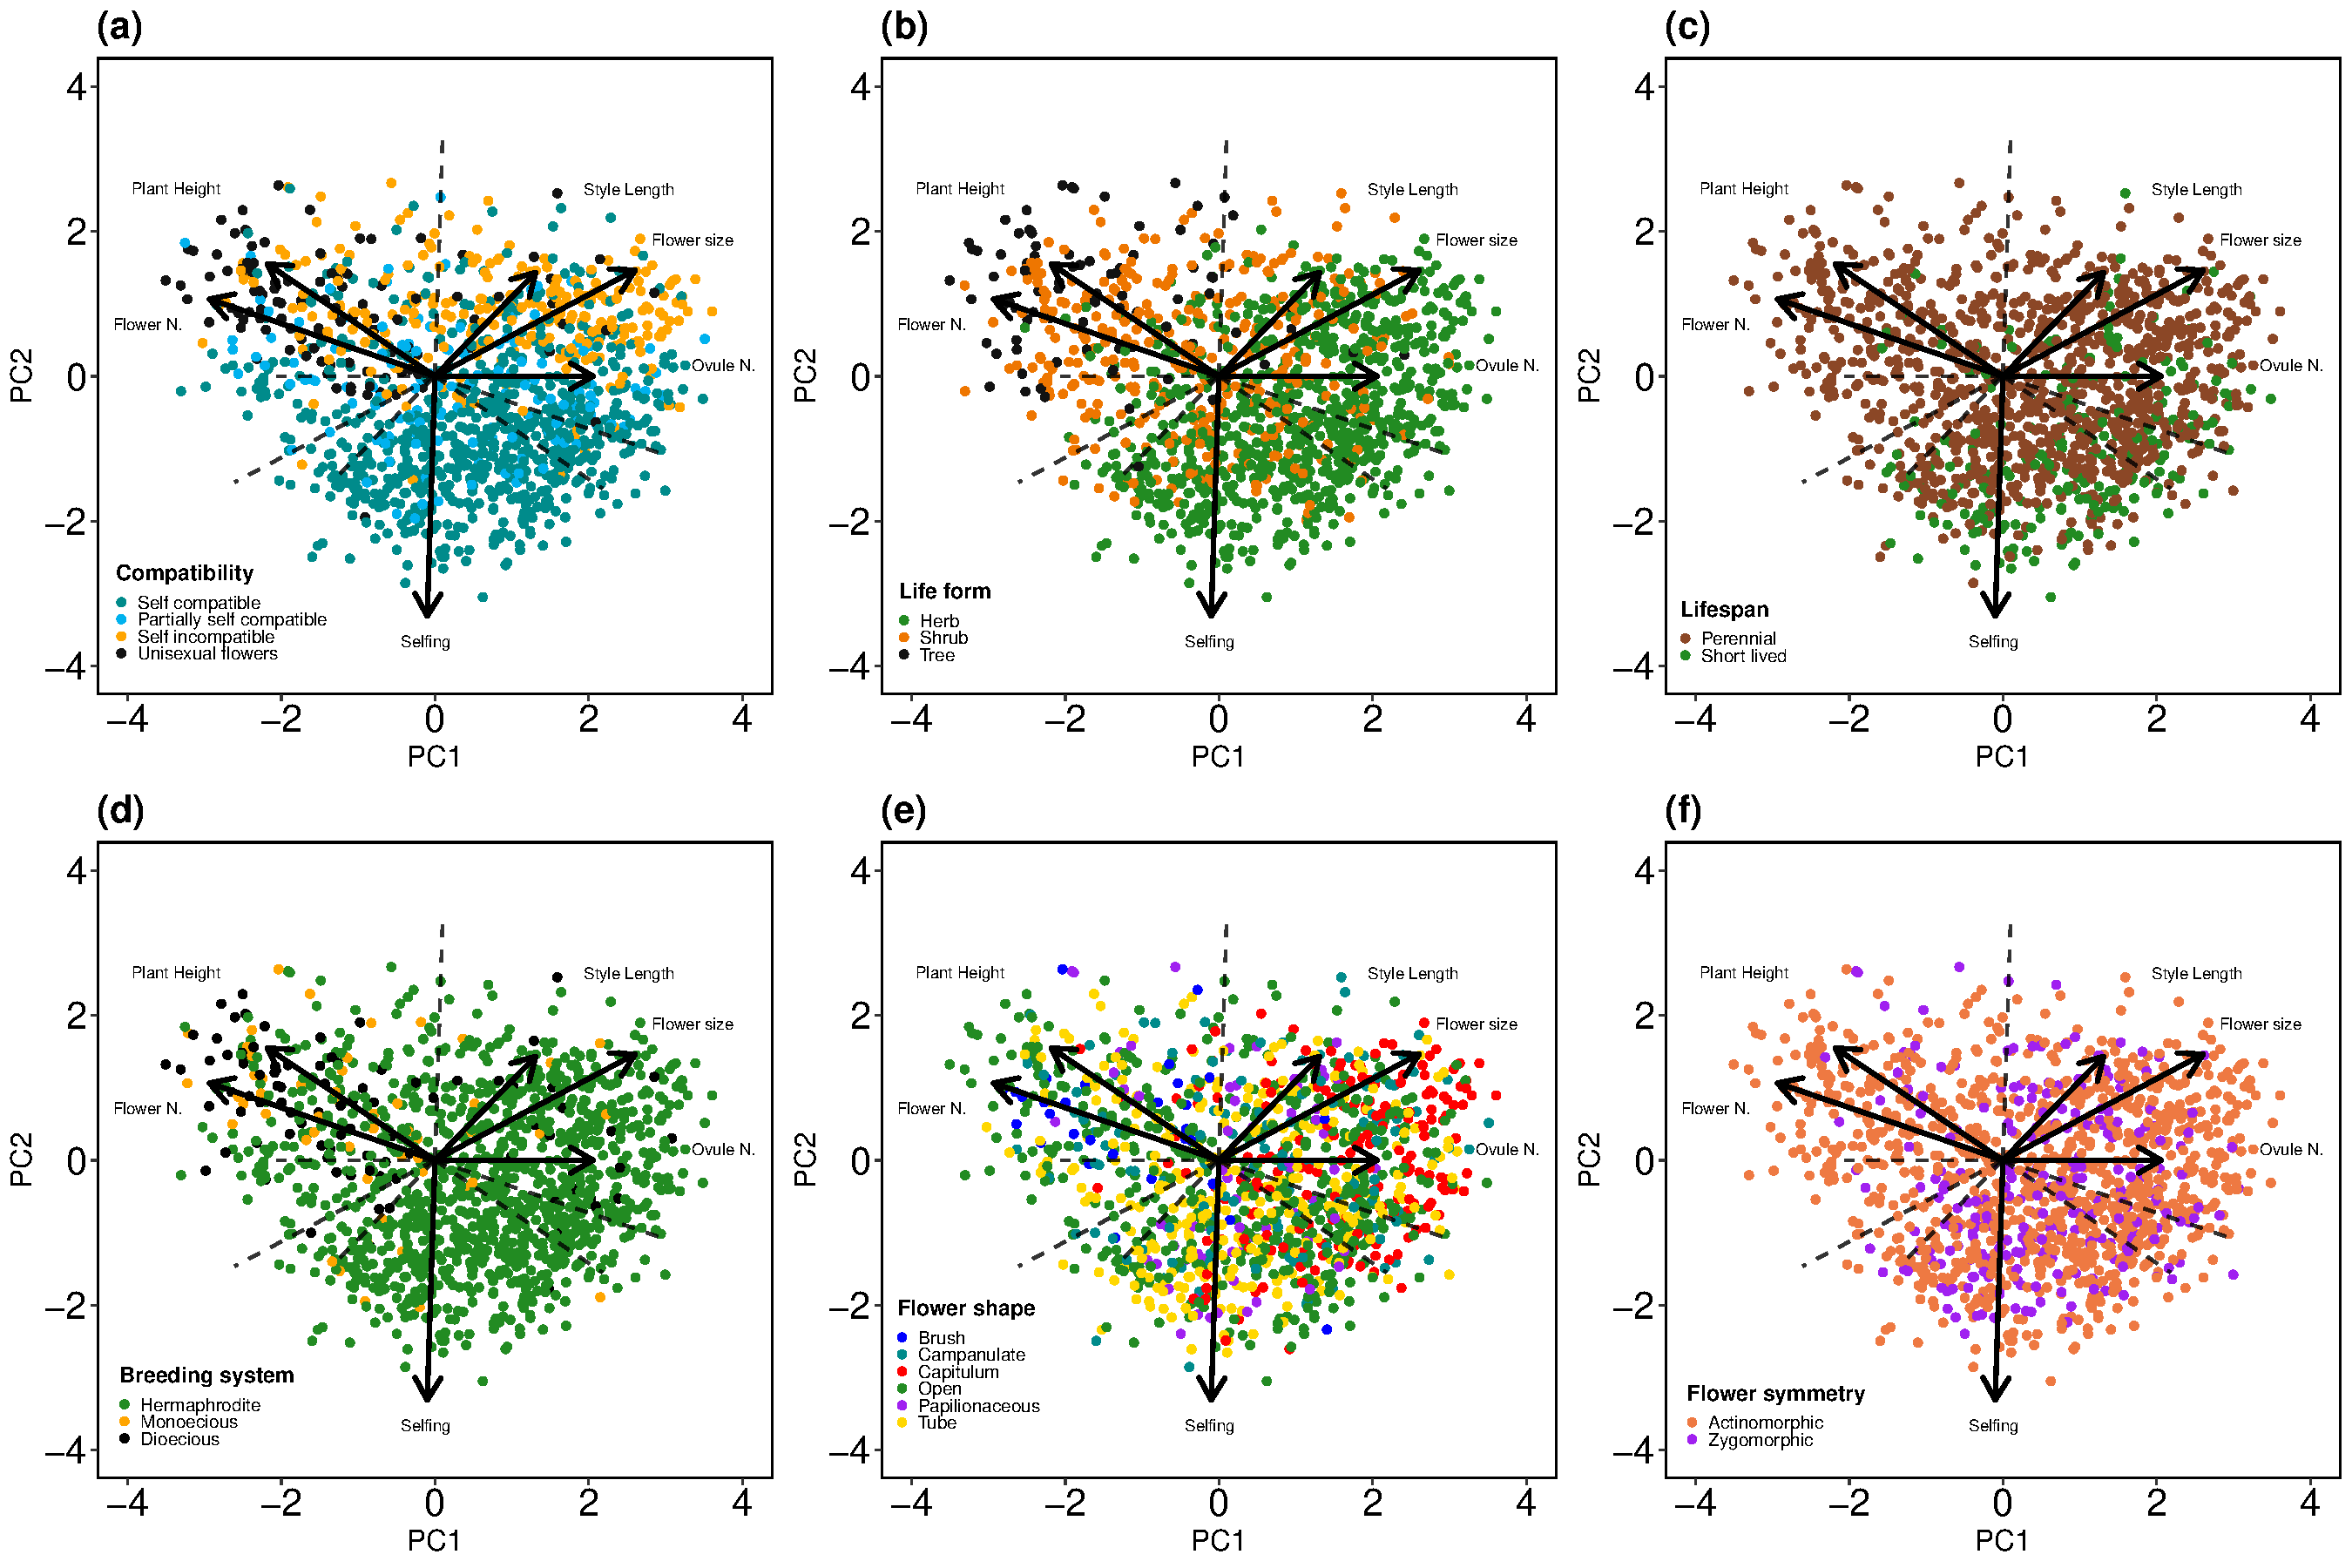
\includegraphics{output/figures/unnamed-chunk-5-1.pdf}
\caption{\label{fig:unnamed-chunk-5}Location of the qualitative traits in
the trait space for traits that showed a statistical association with
the main axis of trait variation. These different traits included:
compatibility system (a), life form (b), lifespan (c), breeding system
(d), flower shape (e) and flower symmetry (f).}
\end{figure}

\subsection{Phylogenetic signal of
traits}\label{phylogenetic-signal-of-traits-1}

We found a strong phylogenetic signal with statistical association (P
\textless{} 0.01) for all quantitative traits (Table S4). The traits
with the highest phylogenetic signal were ovule number (\(\lambda\) = 1)
and plant height (\(\lambda\) = 0.96), followed by flower length
(\(\lambda\) = 0.75), flower width (\(\lambda\) = 0.73) and flower
number per plant (\(\lambda\) = 0.69). Finally the traits that showed
lower phylogenetic signal were inflorescence width (\(\lambda\) = 0.57),
style length (\(\lambda\) = 0.49) and autonomous selfing (\(\lambda\) =
0.34).

Add *pollen and nectar traits

\subsection{Visitation patterns}\label{visitation-patterns}

The overall visitation records of functional groups differed
considerably. There were 2,256 for bees, 1,768 for non-syrphid-Diptera,
845 for syrphids, 437 for Lepidoptera, 432 for Coleoptera and 362 for
non-bee-Hymenoptera. The main axes of trait variation explained little
of the visitation patterns (conditional R2 = 0.31; marginal R2 = 0.06)
but showed interesting trends for the different functional groups
(Figure 3). Furthermore, the additional model with interaction between
the most represented families of Hymenoptera and the main axis of trait
variation (marginal R2 = 0.30; conditional R2 = 0.03) showed that the
family Apidae was the main driver of the observed patterns (Figure S2).
Although Apis mellifera contributed substantially to floral visitation,
the general pattern of bee visitation did not change when A. mellifera
were removed (FSX).

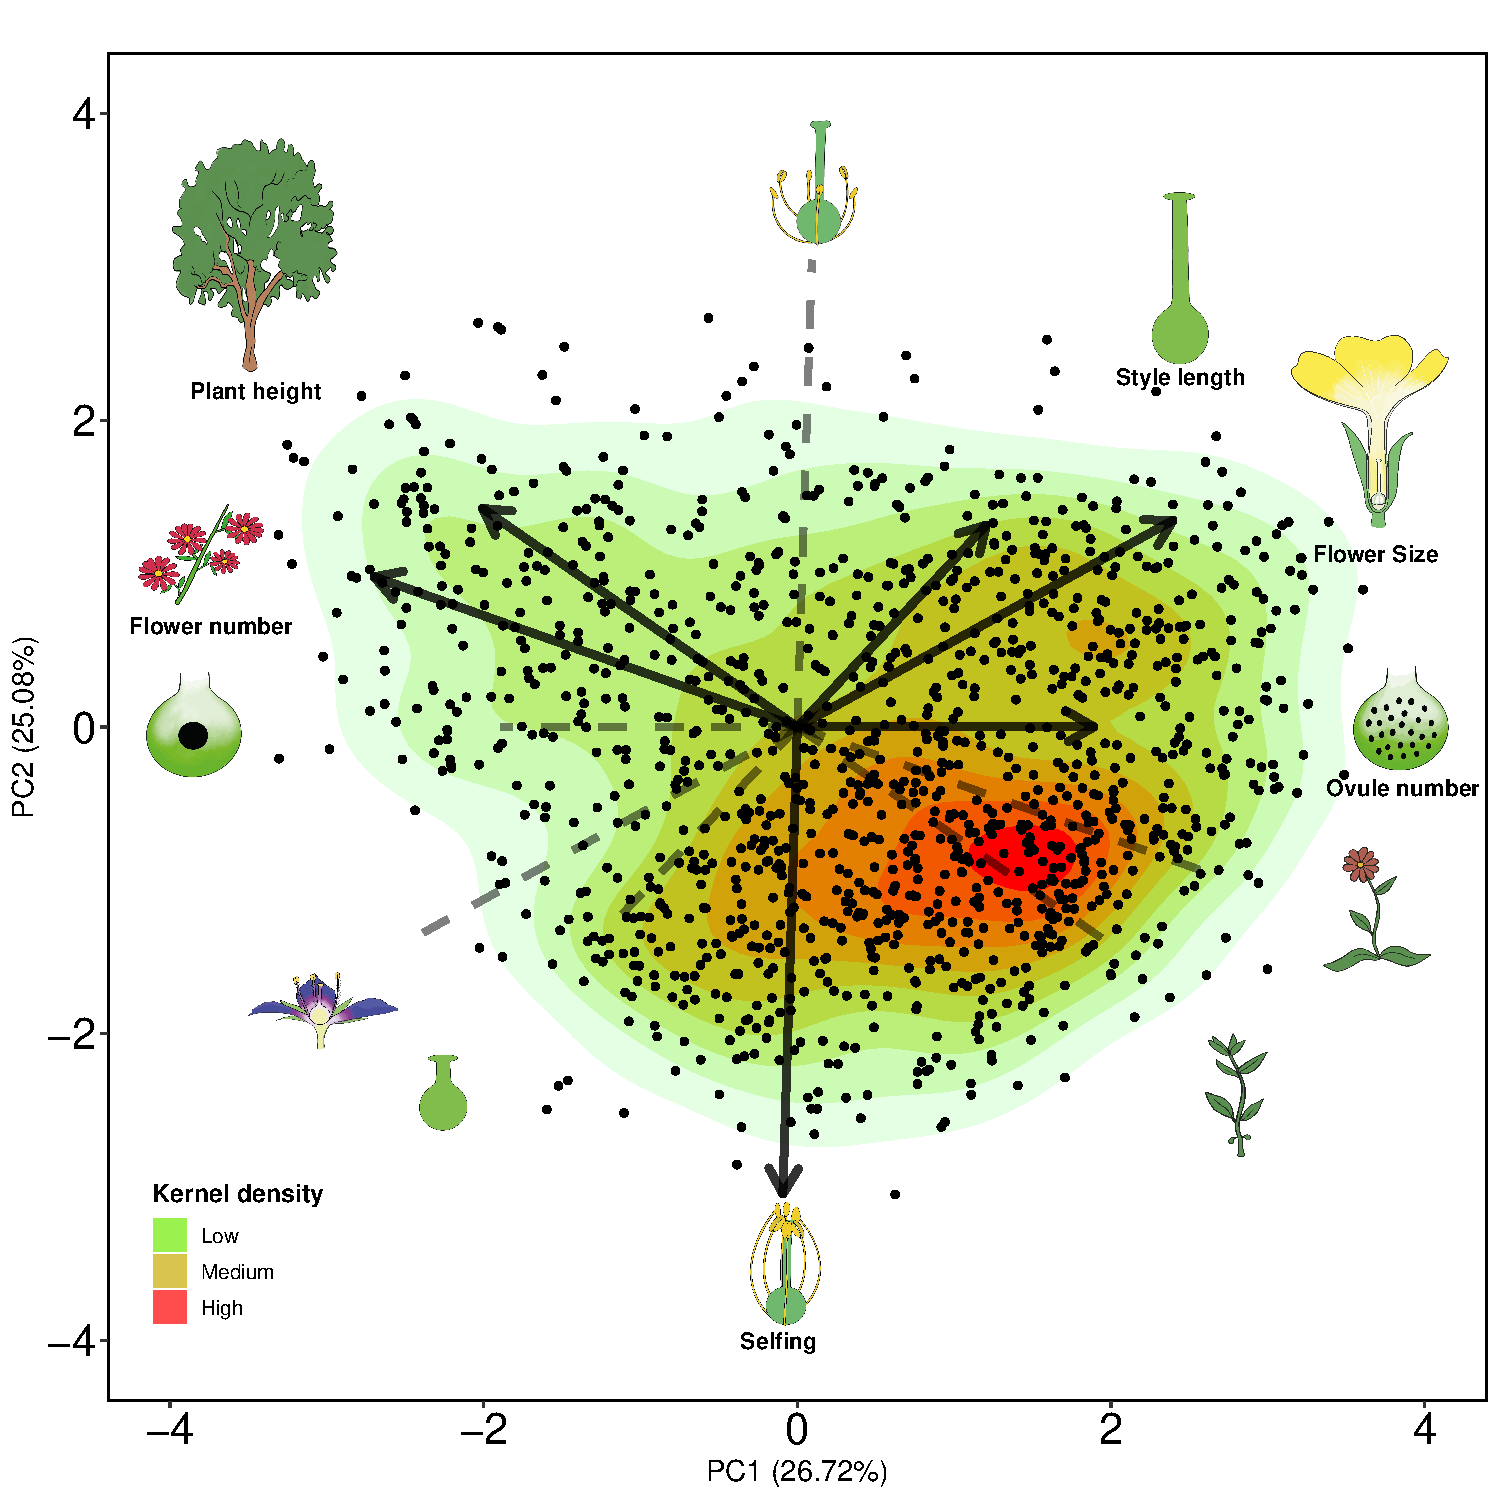
\includegraphics{output/figures/unnamed-chunk-6-1.pdf}

\subsection{Plant species metrics}\label{plant-species-metrics}

The three main axes of trait variation did not explain the position or
role of the plant species in the network (visits \textasciitilde{} PCs:
conditional R2 =0.11 , marginal R2 = 0.02; normalized degree
\textasciitilde{} PCs: conditional R2 =0.24 , marginal R2 = 0.02 and
specialization \textasciitilde{} PCs: conditional R2 =0.37 , marginal R2
= 0.03). However, the functional groups showed different visitation
patterns across the three main axes of trait variation (Figure 3). On
the flower number versus size compromise, all functional groups showed
higher visitation rates on plant species with greater vegetative
investment and more flowers except syrphids which showed the opposite
trend (higher visitation on species with larger flowers and associated
traits). Remarkably, on the pollinator dependence trade-off, all
pollinator functional groups showed an increasing visitation pattern for
species with higher pollinator dependence. Lastly, we found that bees,
Lepidoptera and non-bee Hymenoptera visited more species with larger
style length and Coleoptera, Non-Syrphids Diptera and Syrphids had
greater visitation patterns on species with shorter styles. Furthermore,
with the full model that included all traits, we found that a
considerable amount of variance for plant species network metrics was
explained by the different qualitative and quantitative traits (Visits
\textasciitilde{} Traits: conditional R2 =0.32 , marginal R2 = 0.07;
Normalize degree \textasciitilde{} Traits: conditional R2 =0.46 ,
marginal R2 = 0.16; Specialization \textasciitilde{} Traits: conditional
R2 =0.49, marginal R2 = 0.14).

\section{DISCUSSION}\label{discussion}

Our work highlights that in plant-pollinator networks, plant species
have displayed clear trade-offs in life strategies. These trade-offs can
be differentiated on two main axes of trait variation: the flower
number-size trade-off and the pollinator dependence trade-off. In
addition, we found that relevant qualitative traits were aggregated
within trait space, showing clear delimited strategies of different
plant species within plant-pollinated systems. Moreover, the distinct
pollinator functional groups showed changes in their interaction
strength along these axes of trait variation. Although the main axes of
trait variation explained little the variation of plant species network
metrics, the full model of uncorrelated traits explained partially the
plan level metrics.

\section{CONCLUSIONS}\label{conclusions}

Wrap up

\section{ACKNOWLEDGEMENTS}\label{acknowledgements}

On the shoulders of giants.

\section{REFERENCES}\label{references}

\hypertarget{refs}{}
\hypertarget{ref-abdi2010}{}
Abdi, H., and L. J. Williams. 2010. Principal component analysis. WIREs
Computational Statistics 2:433--459.

\hypertarget{ref-ballantyne2015}{}
Ballantyne, G., K. C. R. Baldock, and P. G. Willmer. 2015. Constructing
more informative plantPollinator networks: Visitation and pollen
deposition networks in a heathland plant community. Proceedings of the
Royal Society B: Biological Sciences 282:20151130.

\hypertarget{ref-barrett2002}{}
Barrett, S. C. H. 2002. The evolution of plant sexual diversity. Nature
Reviews Genetics 3:274--284.

\hypertarget{ref-barrett2003}{}
Barrett, S. C. H. 2003. Mating strategies in flowering plants: The
outcrossing-selfing paradigm and beyond. Philosophical Transactions of
the Royal Society B: Biological Sciences 358:991--1004.

\hypertarget{ref-bartomeus2013}{}
Bartomeus, I. 2013. Understanding Linkage Rules in Plant-Pollinator
Networks by Using Hierarchical Models That Incorporate Pollinator
Detectability and Plant Traits. PLOS ONE 8:e69200.

\hypertarget{ref-bartomeus2016}{}
Bartomeus, I., D. Gravel, J. M. Tylianakis, M. A. Aizen, I. A. Dickie,
and M. Bernard-Verdier. 2016. A common framework for identifying linkage
rules across different types of interactions. Functional Ecology
30:1894--1903.

\hypertarget{ref-baude2016}{}
Baude, M., W. E. Kunin, N. D. Boatman, S. Conyers, N. Davies, M. A.
Gillespie, R. D. Morton, S. M. Smart, and J. Memmott. 2016. Historical
nectar assessment reveals the fall and rise of floral resources in
britain. Nature 530:85--88.

\hypertarget{ref-bluthgen2006}{}
Blüthgen, N., F. Menzel, and N. Blüthgen. 2006. Measuring specialization
in species interaction networks. BMC Ecology 6:9.

\hypertarget{ref-burkner2017}{}
Bürkner, P.-C. 2017. Brms: An R package for Bayesian multilevel models
using Stan. Journal of statistical software 80:1--28.

\hypertarget{ref-carmona2021}{}
Carmona, C. P., R. Tamme, M. Pärtel, F. de Bello, S. Brosse, P.
Capdevila, R. González-M, M. González-Suárez, R. Salguero-Gómez, M.
Vásquez-Valderrama, and A. Toussaint. 2021. Erosion of global functional
diversity across the tree of life. Science Advances 7:eabf2675.

\hypertarget{ref-carvalheiro2014}{}
Carvalheiro, L. G., J. C. Biesmeijer, G. Benadi, J. Fründ, M. Stang, I.
Bartomeus, C. N. Kaiser-Bunbury, M. Baude, S. I. F. Gomes, V. Merckx, K.
C. R. Baldock, A. T. D. Bennett, R. Boada, R. Bommarco, R. Cartar, N.
Chacoff, J. Dänhardt, L. V. Dicks, C. F. Dormann, J. Ekroos, K. S. E.
Henson, A. Holzschuh, R. R. Junker, M. Lopezaraiza-Mikel, J. Memmott, A.
Montero-Castaño, I. L. Nelson, T. Petanidou, E. F. Power, M. Rundlöf, H.
G. Smith, J. C. Stout, K. Temitope, T. Tscharntke, T. Tscheulin, M.
Vilà, and W. E. Kunin. 2014. The potential for indirect effects between
co-flowering plants via shared pollinators depends on resource
abundance, accessibility and relatedness. Ecology Letters 17:1389--1399.

\hypertarget{ref-chamberlain2020}{}
Chamberlain, S., E. Szoecs, Z. Foster, Z. Arendsee, C. Boettiger, K.
Ram, I. Bartomeus, J. Baumgartner, J. O'Donnell, J. Oksanen, B. G.
Tzovaras, P. Marchand, V. Tran, M. Salmon, G. Li, and M. Grenié. 2020.
Taxize: Taxonomic information from around the web.

\hypertarget{ref-chave2009}{}
Chave, J., D. Coomes, S. Jansen, S. L. Lewis, N. G. Swenson, and A. E.
Zanne. 2009. Towards a worldwide wood economics spectrum. Ecology
letters 12:351--366.

\hypertarget{ref-coux2016}{}
Coux, C., R. Rader, I. Bartomeus, and J. M. Tylianakis. 2016. Linking
species functional roles to their network roles. Ecology Letters
19:762--770.

\hypertarget{ref-dellinger2020}{}
Dellinger, A. S. 2020. Pollination syndromes in the 21st century: Where
do we stand and where may we go? New Phytologist 228:1193--1213.

\hypertarget{ref-devaux2014}{}
Devaux, C., C. Lepers, and E. Porcher. 2014. Constraints imposed by
pollinator behaviour on the ecology and evolution of plant mating
systems. Journal of Evolutionary Biology 27:1413--1430.

\hypertarget{ref-diniz-filho2012}{}
Diniz-Filho, J. A. F., L. M. Bini, T. F. Rangel, I. Morales-Castilla, M.
Á. Olalla-Tárraga, M. Á. Rodríguez, and B. A. Hawkins. 2012. On the
selection of phylogenetic eigenvectors for ecological analyses.
Ecography 35:239--249.

\hypertarget{ref-diaz2016}{}
Díaz, S., J. Kattge, J. H. C. Cornelissen, I. J. Wright, S. Lavorel, S.
Dray, B. Reu, M. Kleyer, C. Wirth, I. Colin Prentice, E. Garnier, G.
Bönisch, M. Westoby, H. Poorter, P. B. Reich, A. T. Moles, J. Dickie, A.
N. Gillison, A. E. Zanne, J. Chave, S. Joseph Wright, S. N. Sheremet'ev,
H. Jactel, C. Baraloto, B. Cerabolini, S. Pierce, B. Shipley, D. Kirkup,
F. Casanoves, J. S. Joswig, A. Günther, V. Falczuk, N. Rüger, M. D.
Mahecha, and L. D. Gorné. 2016. The global spectrum of plant form and
function. Nature 529:167--171.

\hypertarget{ref-dormann2008}{}
Dormann, C. F., B. Gruber, and J. Fründ. 2008. Introducing the bipartite
package: Analysing ecological networks. interaction 1.

\hypertarget{ref-fortuna2014}{}
Fortuna, M. A., R. Ortega, and J. Bascompte. 2014. The Web of Life.
arXiv:1403.2575 {[}q-bio{]}.

\hypertarget{ref-fortuna2010}{}
Fortuna, M. A., D. B. Stouffer, J. M. Olesen, P. Jordano, D. Mouillot,
B. R. Krasnov, R. Poulin, and J. Bascompte. 2010. Nestedness versus
modularity in ecological networks: Two sides of the same coin? Journal
of Animal Ecology 79:811--817.

\hypertarget{ref-goodwillie2010}{}
Goodwillie, C., R. D. Sargent, C. G. Eckert, E. Elle, M. A. Geber, M. O.
Johnston, S. Kalisz, D. A. Moeller, R. H. Ree, M. Vallejo-Marin, and A.
A. Winn. 2010. Correlated evolution of mating system and floral display
traits in flowering plants and its implications for the distribution of
mating system variation. The New Phytologist 185:311--321.

\hypertarget{ref-grossenbacher2017}{}
Grossenbacher, D. L., Y. Brandvain, J. R. Auld, M. Burd, P.-O. Cheptou,
J. K. Conner, A. G. Grant, S. M. Hovick, J. R. Pannell, A. Pauw, and
others. 2017. Self-compatibility is over-represented on islands. New
Phytologist 215:469--478.

\hypertarget{ref-hung2018}{}
Hung, K.-L. J., J. M. Kingston, M. Albrecht, D. A. Holway, and J. R.
Kohn. 2018. The worldwide importance of honey bees as pollinators in
natural habitats. Proceedings of the Royal Society B: Biological
Sciences 285:20172140.

\hypertarget{ref-ibanez2012}{}
Ibanez, S. 2012. Optimizing size thresholds in a plant-pollinator
interaction web: Towards a mechanistic understanding of ecological
networks. Oecologia 170:233--242.

\hypertarget{ref-jin2019}{}
Jin, Y., and H. Qian. 2019. V.PhyloMaker: An R package that can generate
very large phylogenies for vascular plants. Ecography 42:1353--1359.

\hypertarget{ref-junker2013}{}
Junker, R. R., N. Blüthgen, T. Brehm, J. Binkenstein, J. Paulus, H. M.
Schaefer, and M. Stang. 2013. Specialization on traits as basis for the
niche-breadth of flower visitors and as structuring mechanism of
ecological networks. Functional Ecology 27:329--341.

\hypertarget{ref-kattge2011}{}
Kattge, J., S. Díaz, S. Lavorel, I. C. Prentice, P. Leadley, G. Bönisch,
E. Garnier, M. Westoby, P. B. Reich, I. J. Wright, J. H. C. Cornelissen,
C. Violle, S. P. Harrison, P. M. V. Bodegom, M. Reichstein, B. J.
Enquist, N. A. Soudzilovskaia, D. D. Ackerly, M. Anand, O. Atkin, M.
Bahn, T. R. Baker, D. Baldocchi, R. Bekker, C. C. Blanco, B. Blonder, W.
J. Bond, R. Bradstock, D. E. Bunker, F. Casanoves, J. Cavender-Bares, J.
Q. Chambers, F. S. C. Iii, J. Chave, D. Coomes, W. K. Cornwell, J. M.
Craine, B. H. Dobrin, L. Duarte, W. Durka, J. Elser, G. Esser, M.
Estiarte, W. F. Fagan, J. Fang, F. Fernández-Méndez, A. Fidelis, B.
Finegan, O. Flores, H. Ford, D. Frank, G. T. Freschet, N. M. Fyllas, R.
V. Gallagher, W. A. Green, A. G. Gutierrez, T. Hickler, S. I. Higgins,
J. G. Hodgson, A. Jalili, S. Jansen, C. A. Joly, A. J. Kerkhoff, D.
Kirkup, K. Kitajima, M. Kleyer, S. Klotz, J. M. H. Knops, K. Kramer, I.
Kühn, H. Kurokawa, D. Laughlin, T. D. Lee, M. Leishman, F. Lens, T.
Lenz, S. L. Lewis, J. Lloyd, J. Llusià, F. Louault, S. Ma, M. D.
Mahecha, P. Manning, T. Massad, B. E. Medlyn, J. Messier, A. T. Moles,
S. C. Müller, K. Nadrowski, S. Naeem, Ü. Niinemets, S. Nöllert, A.
Nüske, R. Ogaya, J. Oleksyn, V. G. Onipchenko, Y. Onoda, J. Ordoñez, G.
Overbeck, W. A. Ozinga, S. Patiño, S. Paula, J. G. Pausas, J. Peñuelas,
O. L. Phillips, V. Pillar, H. Poorter, L. Poorter, P. Poschlod, A.
Prinzing, R. Proulx, A. Rammig, S. Reinsch, B. Reu, L. Sack, B.
Salgado-Negret, J. Sardans, S. Shiodera, B. Shipley, A. Siefert, E.
Sosinski, J.-F. Soussana, E. Swaine, N. Swenson, K. Thompson, P.
Thornton, M. Waldram, E. Weiher, M. White, S. White, S. J. Wright, B.
Yguel, S. Zaehle, A. E. Zanne, and C. Wirth. 2011. TRY a global database
of plant traits. Global Change Biology 17:2905--2935.

\hypertarget{ref-klumpers2019}{}
Klumpers, S. G. T., M. Stang, and P. G. L. Klinkhamer. 2019. Foraging
efficiency and size matching in a plantPollinator community: The
importance of sugar content and tongue length. Ecology Letters
22:469--479.

\hypertarget{ref-lazaro2008}{}
Lázaro, A., S. J. Hegland, and Ø. Totland. 2008. The relationships
between floral traits and specificity of pollination systems in three
Scandinavian plant communities. Oecologia 157:249--257.

\hypertarget{ref-legendre2012}{}
Legendre, P., and L. Legendre. 2012. Numerical ecology. Elsevier.

\hypertarget{ref-moeller2017}{}
Moeller, D. A., R. D. B. Runquist, A. M. Moe, M. A. Geber, C.
Goodwillie, P.-O. Cheptou, C. G. Eckert, E. Elle, M. O. Johnston, S.
Kalisz, R. H. Ree, R. D. Sargent, M. Vallejo-Marin, and A. A. Winn.
2017. Global biogeography of mating system variation in seed plants.
Ecology Letters 20:375--384.

\hypertarget{ref-munoz2016}{}
Munoz, F., C. Violle, and P.-O. Cheptou. 2016. CSR ecological strategies
and plant mating systems: Outcrossing increases with competitiveness but
stress-tolerance is related to mixed mating. Oikos 125:1296--1303.

\hypertarget{ref-novella-fernandez2019}{}
Novella-Fernandez, R., A. Rodrigo, X. Arnan, and J. Bosch. 2019.
Interaction strength in plant-pollinator networks: Are we using the
right measure? PLOS ONE 14:e0225930.

\hypertarget{ref-olesen2007}{}
Olesen, J. M., J. Bascompte, Y. L. Dupont, and P. Jordano. 2007. The
modularity of pollination networks. Proceedings of the National Academy
of Sciences 104:19891--19896.

\hypertarget{ref-ollerton2011}{}
Ollerton, J., R. Winfree, and S. Tarrant. 2011. How many flowering
plants are pollinated by animals? Oikos 120:321--326.

\hypertarget{ref-penone2014}{}
Penone, C., A. D. Davidson, K. T. Shoemaker, M. D. Marco, C. Rondinini,
T. M. Brooks, B. E. Young, C. H. Graham, and G. C. Costa. 2014.
Imputation of missing data in life-history trait datasets: Which
approach performs the best? Methods in Ecology and Evolution 5:961--970.

\hypertarget{ref-peralta2020}{}
Peralta, G., D. P. Vázquez, N. P. Chacoff, S. B. Lomáscolo, G. L. W.
Perry, and J. M. Tylianakis. 2020. Trait matching and phenological
overlap increase the spatio-temporal stability and functionality of
plantPollinator interactions. Ecology Letters 23:1107--1116.

\hypertarget{ref-poisot2016}{}
Poisot, T., B. Baiser, J. A. Dunne, S. Kéfi, F. Massol, N. Mouquet, T.
N. Romanuk, D. B. Stouffer, S. A. Wood, and D. Gravel. 2016. Mangal
making ecological network analysis simple. Ecography 39:384--390.

\hypertarget{ref-rech2016}{}
Rech, A. R., B. Dalsgaard, B. Sandel, J. Sonne, J.-C. Svenning, N.
Holmes, and J. Ollerton. 2016. The macroecology of animal versus wind
pollination: Ecological factors are more important than historical
climate stability. Plant Ecology \& Diversity 9:253--262.

\hypertarget{ref-revell2012}{}
Revell, L. J. 2012. Phytools: An R package for phylogenetic comparative
biology (and other things). Methods in Ecology and Evolution 3:217--223.

\hypertarget{ref-roddy2021}{}
Roddy, A. B., C. Martínez-Perez, A. L. Teixido, T. G. Cornelissen, M. E.
Olson, R. S. Oliveira, and F. A. O. Silveira. 2021. Towards the flower
economics spectrum. New Phytologist 229:665--672.

\hypertarget{ref-salguero2015}{}
Salguero-Gómez, R., O. R. Jones, C. R. Archer, Y. M. Buckley, J.
Che-Castaldo, H. Caswell, D. Hodgson, A. Scheuerlein, D. A. Conde, E.
Brinks, H. de Buhr, C. Farack, F. Gottschalk, A. Hartmann, A. Henning,
G. Hoppe, G. Römer, J. Runge, T. Ruoff, J. Wille, S. Zeh, R. Davison, D.
Vieregg, A. Baudisch, R. Altwegg, F. Colchero, M. Dong, H. de Kroon,
J.-D. Lebreton, C. J. E. Metcalf, M. M. Neel, I. M. Parker, T. Takada,
T. Valverde, L. A. Vélez-Espino, G. M. Wardle, M. Franco, and J. W.
Vaupel. 2015. The compadre Plant Matrix Database: An open online
repository for plant demography. Journal of Ecology 103:202--218.

\hypertarget{ref-salguero2016}{}
Salguero-Gómez, R., O. R. Jones, E. Jongejans, S. P. Blomberg, D. J.
Hodgson, C. Mbeau-Ache, P. A. Zuidema, H. de Kroon, and Y. M. Buckley.
2016. Fast-slow continuum and reproductive strategies structure plant
life-history variation worldwide. Proceedings of the National Academy of
Sciences of the United States of America 113:230--235.

\hypertarget{ref-santos2018}{}
Santos, T., J. A. Diniz-Filho, T. R. e Luis, M. Bini, and M. T. Santos.
2018. Package ``PVR''.

\hypertarget{ref-schiestl2013}{}
Schiestl, F. P., and S. D. Johnson. 2013. Pollinator-mediated evolution
of floral signals. Trends in Ecology \& Evolution 28:307--315.

\hypertarget{ref-smith2018}{}
Smith, S. A., and J. W. Brown. 2018. Constructing a broadly inclusive
seed plant phylogeny. American Journal of Botany 105:302--314.

\hypertarget{ref-stang2006}{}
Stang, M., P. G. L. Klinkhamer, and E. V. D. Meijden. 2006. Size
constraints and flower abundance determine the number of interactions in
a plantFlower visitor web. Oikos 112:111--121.

\hypertarget{ref-stang2009}{}
Stang, M., P. G. L. Klinkhamer, N. M. Waser, I. Stang, and E. van der
Meijden. 2009. Size-specific interaction patterns and size matching in a
plantPollinator interaction web. Annals of Botany 103:1459--1469.

\hypertarget{ref-stekhoven2012}{}
Stekhoven, D. J., and P. Bühlmann. 2012. MissForestNon-parametric
missing value imputation for mixed-type data. Bioinformatics
28:112--118.

\hypertarget{ref-tur2013}{}
Tur, C., R. Castro-Urgal, and A. Traveset. 2013. Linking Plant
Specialization to Dependence in Interactions for Seed Set in Pollination
Networks. PLoS ONE 8:e78294.

\hypertarget{ref-wright2004}{}
Wright, I. J., P. B. Reich, M. Westoby, D. D. Ackerly, Z. Baruch, F.
Bongers, J. Cavender-Bares, T. Chapin, J. H. C. Cornelissen, M. Diemer,
J. Flexas, E. Garnier, P. K. Groom, J. Gulias, K. Hikosaka, B. B.
Lamont, T. Lee, W. Lee, C. Lusk, J. J. Midgley, M.-L. Navas, Ü.
Niinemets, J. Oleksyn, N. Osada, H. Poorter, P. Poot, L. Prior, V. I.
Pyankov, C. Roumet, S. C. Thomas, M. G. Tjoelker, E. J. Veneklaas, and
R. Villar. 2004. The worldwide leaf economics spectrum. Nature
428:821--827.

\eleft

\listoftables

\listoffigures

\section*{SUPPLEMENTARY MATERIAL}\label{supplementary-material}
\addcontentsline{toc}{section}{SUPPLEMENTARY MATERIAL}

\beginsupplement

\end{document}
